%% The following is a directive for TeXShop to indicate the main file
%%!TEX root = Thesis_Driver.tex
\graphicspath{{./Figures/}}
\chapter{Inverse Problem}
\label{ch:Chap3_Inverse}

\section{Regularized inversion} \label{InverseMethod}
In chapter \ref{ch:Chap2_Forward}, I introduced the linear forward calculation for the anomalous magnetic data $\mathbf{b}^{TMA}$ generated by volumes of magnetization.
In a more general case, the discretized system of equations relating the model to the geophysical data can be written as: 
 \begin{equation} \label{linear_system}
  \mathbb{F}[\mathbf{m}] = \mathbf{d} \;,
\end{equation}
where $\mathbb{F}$ is a generic operator relating the geophysical data $\mathbf{d} \in \mathbb{R}^N$ to discrete model parameters $\mathbf{m} \in \mathbb{R}^{nc}$. 
In some cases, $\mathbb{F}$ is linear, but can be non-linear as is the case with amplitude data.
We are usually interested in finding a solution to the inverse problem:
\begin{equation}
\mathbf{m} = \mathbb{F}^{-1}\mathbf{d} \;,
\end{equation}
namely to recover some model parameters $\mathbf{m}$ responsible for a set of observations $\mathbf{d}$.
At this point, the magnetization model $\mathbf{m}$ is general.
In this thesis, $\mathbf{m}$ will take different forms depending on assumptions made, coordinate system chosen or data transformation.  

It is difficult to solve the inverse problem for two reasons. 
First, the inverse problem is often $ill-posed$ as the number of unknown parameters largely exceeds the number of observations. The solution is highly non-unique.
Secondly, field data are generally corrupted by random noise $\mathbf{e}$ such that the true linear system should be written as:
 \begin{equation} \label{linear_system_noisy}
\begin{split}
 \mathbb{F}[\mathbf{m}] = \mathbf{d^{obs}} \\
 \mathbf{d^{obs} = d + e} \;.
\end{split}
\end{equation}
Even if the problem is linear and the matrix $ \mathbb{F}$ is full ranked and invertible, the problem is said to be \emph{ill-conditioned}.
Any solution that satisfies~\ref{linear_system_noisy} is unstable, as small changes in the noise can induce large changes in model values.
Moreover, most geophysical methods have a strong spatial dependency related to the distance between the source and observation location. 
Consequently, few components describing the system $ \mathbb{F}$ can be significantly larger, which can adversely impact numerical solvers.

The inverse problem described by \ref{linear_system_noisy} may admit an infinite number of solutions that are geologically unrealistic, and the solution may not be very stable with respect to the observed data.
As first introduced by \cite{TikhonovArsenin77}, the inverse problem can be formulated as a \emph{regularized} least-squares problem of the form:
\begin{equation}\label{Reg_Least_Squares}
\begin{split}
&\underset{m}{\text{min}} \; \phi(m)  \\
 \phi(m) &= \phi_d \;+\; \beta \phi_m \\
	\phi_d \; &= \;  \|\mathbf{W}_d \left( \mathbb{F}[\mathbf{m}] - \mathbf{d}^{obs} \right)\|_2^2 \\
	\;\phi_m \; &=  \mathbf{R}   \;,
	\end{split}
\end{equation}
where the optimal solution is found at the minimum of the objective function $\phi(m)$. 
The misfit function $\phi_d$ measures the residual between predicted and observed data $\mathbf{d}^{obs}$ normalized by the estimated uncertainties $\mathbf{W}_d$:
\begin{equation}\label{Wd}
\mathbf{W}_d = 
		\begin{bmatrix}
			1/\sigma_1 		& 		0		& \dots  		&  0 \\
			0 		&   	1/\sigma_2	&  0 	&  \vdots \\
			\vdots	&  		 \ddots	&  	   &  0\\
			0 		& 	\dots		& 		0	 &1/\sigma_N 
		 \end{bmatrix} \;,
\end{equation}
where $\sigma_i$ are assigned standard deviations.
Assuming the noise to be Gaussian and uncorrelated, the misfit function follows a chi-squared distribution with an expected value of $N$.
Under this assumption, the expected data misfit is also equal to the number of data $N$.

The model objective function $\phi_m$ is added to stabilize and constrain the solution.
The trade-off parameter $\beta$ balances the relative influence between the misfit function and any \emph{a priori} information prescribed by a chosen regularization $\mathbf{R}$.
There has been much research done on designing robust and effective regularization functions.
In the original magnetic inversion work of \cite{LiOldenburg1996}, the regularization function involves a measure of model \emph{smallness} and \emph{smoothness}.
The general objective function takes the form:
\begin{equation} \label{eq:Phi_int}
\phi(m) =  \phi_d + \beta \Big [ \alpha_s\int_V w_s(r) \; {\left|m(r) - m^{ref}\right|^2} \; dV + 
\sum_{i = x,y,z} \alpha_i \int_V w_i(r)\; {\left|\frac{\partial m(r)}{\partial x_i}\right|^2} \;dV \Big ]\;,
\end{equation}
where $\alpha_s$, $\alpha_x$, $\alpha_y$ and $\alpha_z$ are adjustable constants balancing the relative contribution between the various components of the model objective function.
The first integral measures the deviation from a reference model $m^{ref}$. The three following integrals measure the spatial gradients of the model $m(r)$ in Cartesian coordinates. 
The weighting functions ${w_s(r)},\;{w_x(r)}, {w_y(r)}$ and ${w_z(r)}$ are cell-based penalties added to the system to reflect specific characteristics expended from the solution.
For potential field problems, it is common to resort to a sensitivity-based weighting in order to compensate for the natural decay of the kernel functions, such that:
\begin{equation}\label{Cell-weight}
\begin{split}
w_s(r) = w_r(r) \; \tilde w_s(r) \\
w_i(r) = w_r(r) \; \tilde w_i(r) \;,\\
\end{split}
\end{equation}
where $w_r(r)$ is a general distance weighting, and $\tilde w_s$, $\tilde w_i$ are customizable weights that reflect any available $a \; priori$ information.
Note that the distance weighting $w_r(r)$ is applied through the regularization function rather than directly to the sensitivity matrix as prescribed by \cite{LiOldenburg1996}. 
Reasons for this change will be discussed in Section~\ref{Wr_Section} while experimenting with different $l_p$-norm regularization functions. 

I discretize~\ref{eq:Phi_int} on a tensor mesh made of rectangular prims such that:
 \begin{equation} \label{eq:Phi_disc}
\phi(m) =  \phi_d + \beta \Big [ {\| \mathbf{W}_s \;( \mathbf{m - m^{ref}})\|}^2_2  + \sum_{i = x,y,z}  {\|   \mathbf{W}_i  \; \mathbf{G}_i \; \mathbf{m}\|}^2_2  \Big ]\;,
\end{equation}
where the diagonal matrices $\mathbf{W}_s$ and $\mathbf{W}_i \in \mathbb{R}^{nc \times nc}$ contain dimensional scales that arise from the  discretization and cell-based weights (${w}_s(r)$, ${w}_i(r)$).
The global scaling constants $\alpha_s$ and $\alpha_x$ are also absorbed as cell weights. 
The measure of spatial gradients are calculated by a generic forward difference scheme such that:
\begin{equation}\label{1D_Grad}
\mathbf{G}_i = 
		\begin{bmatrix}
			-1 		& 		1	&  	0		& \dots  		&  0 \\
			0 		& 	\ddots	&  	 \ddots	&  \ddots  	&  \vdots \\
			\vdots	&  		 \ddots	&  0	& -1 &  1\\
			0 		& 	\dots		& 		0	& 1 &  -1 
		 \end{bmatrix}\;,
\end{equation}
where the gradient operator $\mathbf{G}_i \in \mathbb{R}^{nc \times nc}$ calculates the horizontal changes in model parameters $\mathbf{m}$. 
I voluntarily removed all spatial dimensions out of the gradient operators for reasons that will be discussed in Section \ref{Wr_Section}.
The last row is using a backward difference in order to get a square matrix.
The banding structure of the gradient operators is different for $\mathbf{G}_x$, $\mathbf{G}_y$ and $\mathbf{G}_z$ to account for the ordering of the cells in the tensor mesh. 

For ease of notation, I write the model objective function in compact form as:
\begin{equation}
\phi_m = {\|\mathbf{W}_m\left(\Delta \mathbf{m} \right)\|}_2^2 \;,
\end{equation}
such that:
\begin{equation*}
\mathbf{W_\text{m}^TW_\text{m}} = \mathbf{W_\text{s}^TW_\text{s}} +  \sum_{i = x,y,z} \mathbf{G_\text{i}^TW_\text{i}^TW_\text{i}G_\text{i}} \;,
\end{equation*}
as well as:
\begin{equation*}
\Delta \mathbf{m} = \mathbf{m}-\mathbf{m}^{ref}\;,
\end{equation*}
to define the deviation between the model parameters $\mathbf{m}$ and the reference model $\mathbf{m}^{ref}$.
\subsection{Iterative solver}\label{Iterative solver}
As previously stated, my goal is to minimize the objective function described by \ref{eq:Phi_disc}.
The minimum solution is found where the partial gradients of the function are vanishing such that:
\begin{equation}
\mathbf{g(m)} = \frac{\partial \phi(m)}{\partial m} = 0 \;.
\end{equation}
Taking the partial derivatives of \ref{eq:Phi_disc} with respect to the model parameters yield:
\begin{equation}\label{eq:dphi_dm_nonlin}
\mathbf{J^T W_\text{d}^T W_\text{d}} \left[ \mathbb{F}[\mathbf{m}] -\mathbf{d}^{obs} \right]+ \beta \mathbf{W^T}_m \mathbf{W}_m  \left( \Delta \mathbf{m} \right)=0  \;,
\end{equation}
where $\mathbf{J}$ is the Jacobian of the forward operator:
\begin{equation}
\mathbf{J} = \frac{\partial  \mathbb{F}[\mathbf{m}]}{\partial \mathbf{m}} \;.
\end{equation}

More generally, we are interested in solving the nonlinear system described by \ref{eq:dphi_dm_nonlin}, which can be done with second-order methods. 
Newton's method computes a series of model updates $\delta \mathbf{m}$ by solving the system:
\begin{equation}
\mathbf{H} \; \delta \mathbf{m} = -\mathbf{g(m}^{(j)}) \;,
\end{equation}
where $\mathbf{H}$ is the Hessian, or second-order derivatives of the objective function.
The optimization problem is solved iteratively such that:
\begin{equation}
\mathbf{m}^{(j+1)} = \mathbf{m}^{(j)} + \alpha \delta \mathbf{m} \;,
\end{equation}
where the superscript $(j)$ denotes the solver iterations for a model perturbation $\delta \mathbf{m}$ scaled by a step length $\alpha$.

Computing the true Hessian can be computationally expensive.
For least-squares problems, the Gauss-Newton method can be used to approximate the Hessian such that:
\begin{equation}\label{Hessian}
\frac{\partial^2 \phi}{\partial m^2} \approx \mathbf{\tilde H} =   \mathbf{J^T W_\text{d}^T W_\text{d} J} +  \beta \mathbf{W^T}_m \mathbf{W}_m \;,
\end{equation}
where the assumption is made that the change in Jacobian is small between each iteration:
\begin{equation}
\mathbf{J(m}^{(j)} + \delta \mathbf{m}) \approx \mathbf{J(m)}^{(j)}\;,
\end{equation}
and that the model update is approximated to be along the gradient direction such that:
\begin{equation}
\mathbf{\mathbb{F}[m + \delta m]} \approx \mathbb{F}[\mathbf{m}] + \mathbf{J \delta m}\;.
\end{equation}
Combining \ref{eq:dphi_dm_nonlin} and \ref{Hessian}, and ignoring the superscript $(j)$ yields:
\begin{equation}\label{GaussNewt}
\begin{aligned}
 \mathbf{\tilde H}\; \delta \mathbf{m} &= -\mathbf{g(m)})  \\
\left (\mathbf{J^T W_\text{d}^T W_\text{d} J} + \beta \mathbf{W^T}_m \mathbf{W}_m \right) \delta \mathbf{m} &= \\
&- \mathbf{J^T W_\text{d}^T W_\text{d}} \left[ \mathbb{F}[\mathbf{m}] -\mathbf{d}^{obs} \right] - \beta\mathbf{W^T}_m \mathbf{W}_m  \left( \Delta \mathbf{m} \right)\;.
\end{aligned}
\end{equation}

Solving \ref{GaussNewt} gives a step direction. 
Each Gauss-Newton step requires a solution to linear system of the form $\mathbf{A\;x\;=b}$.
In our case, the left-hand-side of \ref{GaussNewt} can be assumed to be a symmetric positive definite matrix. Hence it is possible find a unique solution by directly computing the inverse of the pseudo-Hessian. 
From a practical standpoint however, the computational cost of this operation on a dense matrix is $O(nc^3)$, which can rapidly become prohibitive for a large system of equations.

Krylov Space methods have been proposed as an alternative to direct solvers.
Iterative solvers, such as the Conjugate Gradient (CG) method, apply a series of orthogonal steps towards the minimum of a function.
Each step is said to be $A$-orthogonal to the previous ones, contributing to the fast convergence of CG over simpler gradient descent methods. 
The reader is encouraged to read \cite{Shewchuk1994} for a comprehensive review of the method.
The algorithm is presented in Table~\ref{CG}.
It can be shown that for a symmetric positive definite matrix $\mathbf{A}$, the CG method converges to a unique solution in at most $O(nc)$ operations.
It is rarely required to solve the system exactly however.
My algorithm uses a stopping criteria for the minimum CG update  ($\delta > 1e-4$), after which a Gauss-Newton step direction $\delta \mathbf{m}$ is returned.  
The step length $\alpha$ is calculated by a line-search method as presented in Table~\ref{tbl:Line-search}.
\begin{table}[h!]
\centering
\caption{Conjugate Gradient algorithm}
\label{CG}
\renewcommand{\arraystretch}{1.2}
\begin{tabular}{|c|}\hline
\textbf{Initialize}: $\mathbf{d}_{(0)} = \mathbf{r}_{(0)} = \mathbf{b} - \mathbf{A\;x}_{(0)}$ \\ \hline
$while: \; \|r\| > \delta$ \\ 
$\alpha_{(i)} = \frac{\mathbf{r}_{(i)}^T \mathbf{r}_{(i)}}{\mathbf{d}_{(i)}^T\mathbf{A\;d}_{(i)}}$ \\
$\mathbf{x}_{(i+1)} = \mathbf{x}_{(i)} + \alpha_{(i)} \mathbf{d}_{(i)}$ \\
$\mathbf{r}_{(i+1)} = \mathbf{r}_{(i)} - \alpha_{(i)} \mathbf{Ad}_{(i)}$ \\
$\beta_{(i+1)} = \frac{\mathbf{r}_{(i+1)}^T \mathbf{r}_{(i+1)}}{\mathbf{r}_{(i)}^T\mathbf{r}_{(i)}}$ \\
$\mathbf{d}_{(i+1)} = \mathbf{r}_{(i+1)} + \beta_{(i+1)} \mathbf{d}_{(i)}$ \\ \hline
\end{tabular}
\end{table}
\begin{table}[h!]
\centering
\caption{Line-search}
\label{tbl:Line-search}
\renewcommand{\arraystretch}{1.2}
\begin{tabular}{|c|}\hline
\textbf{Initialize}:   $\alpha = 1\;,\;\mathbf{\hat m = m^{(j)}}$\\ \hline
$while : \phi(\mathbf{\hat m) \ge \phi(m^{(j)}})$ 	\\
	 $\alpha = \alpha / 2 $\\
	 $ \mathbf{\hat m = m^{(j)} + \alpha \delta m}$\\  \hline
 $\mathbf{m^{(j+1)} = \hat m }$\\ \hline
\end{tabular}
\end{table}
The Gauss-Newton steps are repeated until the model updates falls below some threshold value, $|\alpha \delta \mathbf{m}| < \gamma$,
where $\gamma$ is some small value. In this thesis, I fix $\gamma=1e-4$, which experimentally has proven to be a good compromise between computation cost and accuracy.

In order to reduce the amount of memory required to store the dense matrix $ \mathbf{\tilde H}$ in~\ref{GaussNewt}, the Gauss-Newton steps can be formulated as an overdetermined problem of the form:
 \begin{equation}\label{eq:lsqr_dphi_dm}
 \begin{bmatrix}
\mathbf{W}_d \;\mathbf{J} \\
\sqrt{\beta} \mathbf{W}_s \\
\sqrt{\beta} \mathbf{W}_x \;\mathbf{G}_x \\
\sqrt{\beta} \mathbf{W}_y \;\mathbf{G}_y  \\
\sqrt{\beta} \mathbf{W}_z \;\mathbf{G}_z 
 \end{bmatrix} \delta \mathbf{m} =
  - \begin{bmatrix}
\mathbf{W}_d \;\left( \mathbb{F}[\mathbf{m}] - \mathbf{d}^{obs} \right)\\
\mathbf{W}_s \left( \Delta \mathbf{m} \right) \\
\mathbf{W}_x \;\mathbf{G}_x \left( \Delta \mathbf{m} \right)\\
\mathbf{W}_y \;\mathbf{G}_y \left( \Delta \mathbf{m} \right)\\
\mathbf{W}_z \;\mathbf{G}_z \left( \Delta \mathbf{m} \right)
 \end{bmatrix} \;.
 \end{equation}
The CG steps presented in Table~\ref{CG} are altered slightly in order to calculate the residual $\mathbf{r}_{(i)}$ and descent direction $\mathbf{d}_{(i)}$.
Memory savings are important as I avoid forming a dense system  $\mathbf{\tilde H} \in \mathbb{R}^{nc \times nc}$, but only require sparse matrix-vector products.

\subsection{Preconditioner}
As explained in Section~\ref{Iterative solver}, I want to solve iteratively a normal equation of the form $\mathbf{Ax=b}$. The performance of iterative solvers depends strongly on the condition number $\kappa$ of the left-hand side matrix $\mathbf{A}$ such that:
\begin{equation}
\kappa = \frac{\lambda_{max}}{\lambda_{min}}\;,
\end{equation}
where $\lambda_{max}$ and $\lambda_{min}$ are the largest and and smallest eigenvalues of $\mathbf{A}$.
It can be shown that an upper bound on the convergence rate of CG is function of this condition number such that:
\begin{equation}
\omega \le \frac{\kappa -1}{\kappa+1}\;,
\end{equation}  
where the convergence rate $\omega$ gets worse as the condition number increases.
In order to accelerate the convergence, it is common to resort to a \emph{preconditioner} to improve the spectral properties of $\mathbf{A}$ \cite[]{Vorst2003}.
The basic idea is to pre-multiply the linear system such that:
\begin{equation}
\mathbf{P\;Ax = P\;b}\;,
\end{equation} 
where the resulting condition number of $\mathbf{P\;A}$ is smaller than the original matrix $\mathbf{A}$. 
Assuming that $\mathbf{A}$ is invertible, the perfect preconditioner is its inverse $\mathbf{A}^{-1}$, in which case  $\mathbf{A^{-1} A}$ is the identity matrix with a condition number of 1. 
Computing this preconditioner would obviously be redundant, since if I know $\mathbf{A}^{-1}$, then I would have already solved the problem.

I can decompose the matrix $\mathbf{A}$ in its lower and diagonal blocks:
\begin{equation}
\mathbf{A} =\mathbf{L + D + L^T}\;,
\end{equation} 
where in our case the matrix $\mathbf{D}$ is the diagonal of the pseudo Hessian described by Equation~\ref{GaussNewt}. The Jacobi preconditioner is the simplest choice where I set $\mathbf{P = D^{-1}}$.
In this research project, the matrix $\mathbf{A}$ is a positive definite matrix, hence $\mathbf{D}$ is assumed to have diagonal elements that are strictly non-zero positive numbers. The preconditioning matrix $\mathbf{P}$ is updated before each Gauss-Newton step and pre-multiplied ahead of the Conjugate Gradient solver presented in Table~\ref{CG}. 

\subsection{Bound constraints}
In many cases, the solution $\mathbf{m}$ is expected to be bounded on a specific interval.
In particular for the magnetic problem, the magnetic susceptibility $\kappa$ can only be a positive real number on the interval $\kappa_i \in [0,\infty)$.
Three strategies have been proposed in the literature.
In \cite{LiOldenburg03}, positive constraints are applied via a log-barrier penalty term such that:
\begin{equation}
\phi(\lambda) = \phi_d + \beta \phi_m - 2\lambda \sum_{i=1}^{nc} ln(\kappa_i) \; ,
\end{equation}
where the log barrier parameter $\lambda$ controls the influence of the logarithmic penalty function.
The method solves a series of non-linear problems by monotonically reducing $\lambda$ until convergence to a stable solution has been reached.
As $\kappa_i \rightarrow 0$, the $log(\kappa_i)$ tends to be large and negative, hence strongly penalized during the minimization process. 
The same approach can be used to impose and upper bound on the model parameters.

In a second approach, the model values are parameterized into a quantity that can only be positive.
\cite{LelievreMSc} proposes transforming the model parameters such that:
\begin{equation}
m_i = \kappa_i^{(1/2)}\:,
\end{equation}
in which case if $m_i \in (-\infty,\infty),$ then $\kappa_i \in [0,\infty)$, hence a strictly positive value. 
This method has the advantage of reducing the size of the system to be solved, but can only be used as a lower bound.

The third strategy, which is used in this work, is the Projected Gradient method as presented in \cite{Vogel02}.
Within the line-search algorithm presented in Table~\ref{tbl:Line-search}, model parameters outside the bounds are replaced and set to be inactive for the following Gauss-Newton iteration. 

All three strategies make the inverse problem non-linear with respect to $\mathbf{m}$. The Projected Gauss-Newton method is the simplest to implement however within an iterative solver framework.
It does not require additional parameters to be adjusted and can be used to impose both an upper and a lower bound. All the algorithms presented in this thesis were implemented with the Projected Gauss-Newton method.

\newpage
\section{Magnetic susceptibility inversion}\label{ch:Chap3_MSI}
As formulated in~\ref{bTMI}, the observed Total Magnetic Anomaly data $\mathbf{b}^{TMA}$ are related to discrete magnetization parameters $\vec {\mathbf{M}}$ by a large under-determined system of equations $\mathbf{P\;T} \in \mathbb{R}^{N \times (3*nc)}$.
A long standing strategy, as adopted by \cite{LiOldenburg1996}, \cite{Pilkington97} and others, is to neglect the effect of self-demagnetization and remanence and invert directly for the magnetic susceptibility of rocks. 
Assuming a uniform magnetization direction parallel to the Earth's field $\vec H_0$, the linear system \ref{b_explicit} can be written as:
\begin{equation}\label{b_MAG3D}
\begin{split}
	b_{x} &= \left[\;T_{xx}\;H_{0_x} + T_{xy}\;H_{0_y}  + T_{xz}\;H_{0_z}  \;\right] \kappa \\
	b_{y} &= \left[\;T_{xx}\;H_{0_x} + T_{xy}\;H_{0_y}  + T_{xz}\;H_{0_z}  \;\right] \kappa \\
	b_{z} &= \left[\;T_{xx}\;H_{0_x} + T_{xy}\;H_{0_y}  + T_{xz}\;H_{0_z}  \;\right] \kappa \;,
\end{split}
\end{equation}
where the magnetic field response is linearly related to the effective susceptibility parameter $\kappa$.
For a larger system involving $N$ observations over a model space discretized into $nc$ cells, \ref{b_MAG3D} is written as:
\begin{equation} 
	\begin{split}
	\mathbf{b}^{TMA} =& \mathbf{P\;T\;H} \; \boldsymbol{\kappa} \\
	\mathbf{H} = 
	\begin{bmatrix}
	H_{0_x}\mathbf{I} \\
	H_{0_y}\mathbf{I} \\
	H_{0_z}\mathbf{I}
	\end{bmatrix} 
	\;\;&,\;\; \boldsymbol{\kappa} = 
	\begin{bmatrix}
		\kappa_1 \\
		\kappa_2 \\
		\vdots 	 \\
		\kappa_{M} 
	\end{bmatrix} \\ \\
	\mathbf{H} \in \mathbb{R}^{(3nc) \times nc} \;,&\; \boldsymbol{\kappa} \in \mathbb{R}^{nc} \;,
	\end{split}
\end{equation}
where $\mathbf{I}$ is the identity matrix and $\mathbf{H}$  is a block diagonal matrix containing the orientation of the inducing field $\vec H_0$ in Cartesian coordinates.
Since the inducing field $\vec H_0$ is assumed to be constant, the matrix product  $\mathbf{P\;T\:H}$ can be directly incorporated into a linear system of equations such that:
\begin{equation} \label{Fwr_susc}
\mathbf{b}^{TMA} = \mathbf{F} \;  \boldsymbol{\kappa}  \;,
\end{equation}
where  $\mathbf{F} \in \mathbb{R}^{(N) \times nc}$ is the linear forward operator relating the discrete magnetic susceptibility values $\kappa$ to the magnetic field observations $\mathbf{b}^{TMA}$.

\subsection{Synthetic example}\label{Induced Mag}
Having defined the linear system relating the anomalous field data  $\mathbf{b}^{TMA}$ to a discrete magnetic susceptibility model $\boldsymbol{\kappa}$, I illustrate the forward calculation with a synthetic example shown in Figure \ref{fig:3D_Model_INDUCED}.
The model consists of a folded anomaly with induced magnetization of 3 A/m, arching around a discrete block with magnetization of 2 A/m. The arc-shaped anomaly dips $20^\circ$ towards the south. 
From the relation between induced magnetization and ambient field:
\begin{equation}
\vec M_{ind} = \kappa \vec B_0 / \mu_0 \;,
\end{equation}
 the susceptibility of both anomalies are 0.075 and 0.05 SI respectively, subject to a 50,000 nT inducing field $\vec H_0$.
I create this model in order to simulate complex geology with varying shapes and depth extent.
The model is discretized  on a uniform 20 meters cell size mesh.
A grid of 342 observation stations is placed on a plane 20 meters above the top of the mesh.
I generate $\mathbf{b}^{TMA}$ data using \ref{Fwr_susc} as shown in Figure \ref{fig:3D_Data_INDUCED}.
Data are corrupted with random Gaussian noise, 1 nT standard deviation, to simulate field data conditions.
\begin{figure}[h!]
\centering
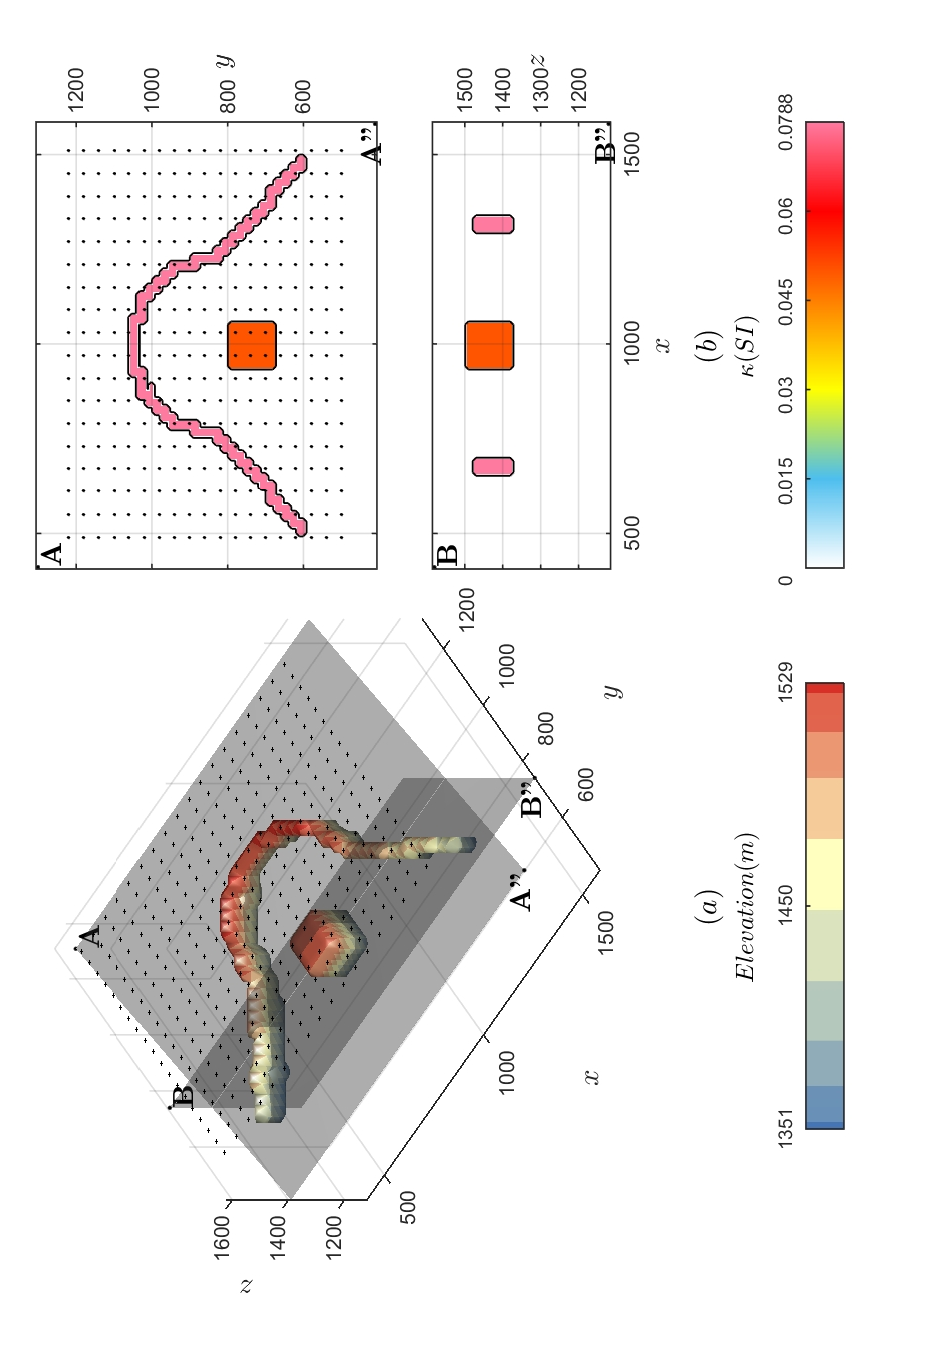
\includegraphics[scale=0.52, angle =270]{3D_Model_INDUCED.pdf}
\caption{ $\bf{(a)}$ Synthetic susceptibility model consisting of a folded anomaly ($\kappa=0.075 $ SI) arching around a discrete block ($\kappa=0.05 $ SI)  . }
\label{fig:3D_Model_INDUCED}
\end{figure}
\begin{figure}[h!]
\centering
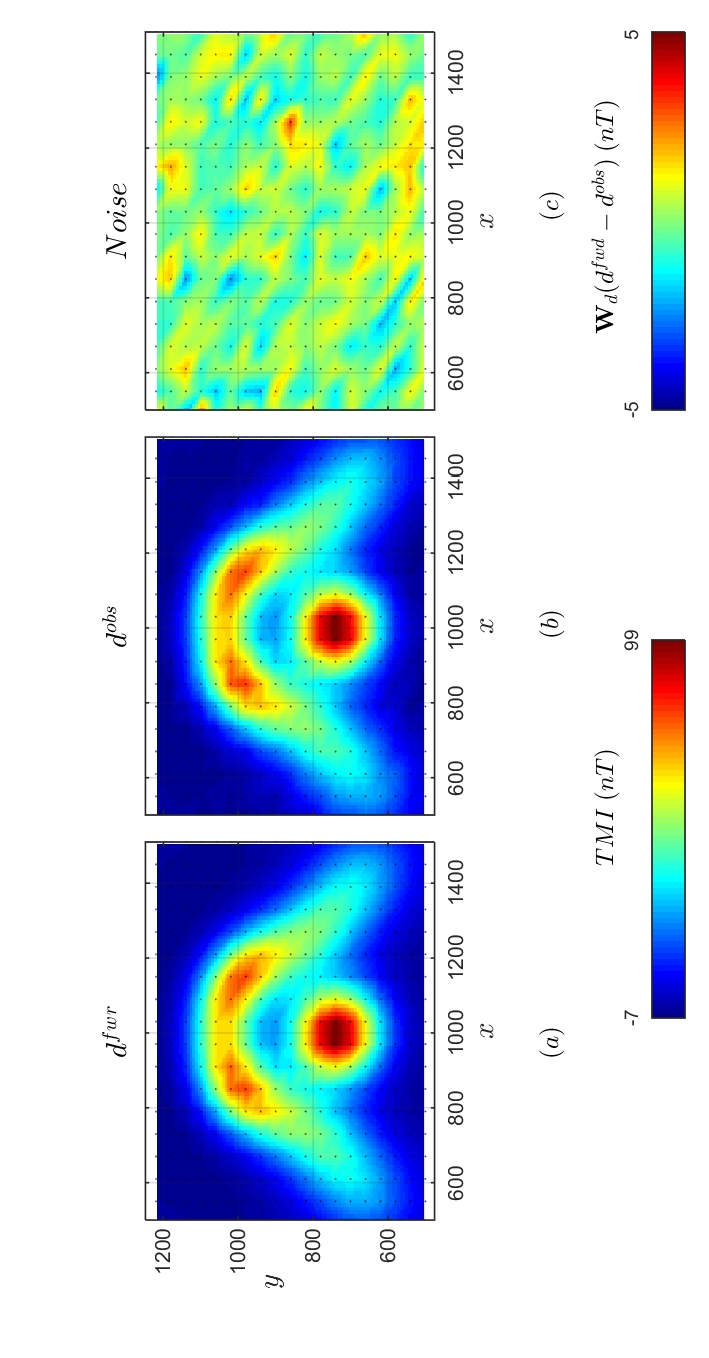
\includegraphics[scale=0.52, angle =270]{3D_Data_INDUCED.pdf}
\caption{ $\bf{(a)}$ Data generated from the synthetic susceptibility model subject to a vertical 50,000 nT inducing field. (b) Data are then corrupted with (c) random Gaussian noise, 1 nT standard deviation.}
\label{fig:3D_Data_INDUCED}
\end{figure}

I then follow with the inverse problem, namely to recover a distribution of susceptibility values from the $\mathbf{b}^{TMA}$ data as presented in \cite{LiOldenburg1996}. 
Similar to the general system~\ref{Reg_Least_Squares}, the objective function to be minimized is written as:
 \begin{equation} \label{eq:phi_3D}
\begin{aligned}
&\phi(\kappa) =  \|\mathbf{W_\text{d} (\;F\kappa - d}^{obs}\;)\|_2^2 + \beta \| \mathbf{W}_m \kappa \|^2_2\;.
\end{aligned}
\end{equation}
In this case, $\mathbf{W}_d$ is simply the identity matrix since the noise is known to have a standard deviation of exactly one.
I also set the reference mode $\mathbf{m}^{ref}$ to zero, hence forcing the solution to be $small$ and $smooth$.
Table~\ref{tbl:Induced_inv} summarizes the inversion parameters used.

\begin{table}
\centering
\caption{Inversion parameters.}
\label{tbl:Induced_inv}
\renewcommand{\arraystretch}{1.2}
\begin{tabular}{|c|c|}
Core cell size & $20\times20\times20$ m \\
nc cells & 82,000\\
N data& 342 \\
$\alpha_s,\; \alpha_x,\; \alpha_y, \; \alpha_z$ & 2.5e-3, 1, 1, 1 \\
$w_s,\; w_x,\; w_y, \; w_z$ & 1, 1, 1, 1 \\
Uncertainties & 1 nT
\end{tabular}
\end{table}

I minimize~\ref{eq:phi_3D} iteratively following the procedure presented in Section~\ref{Iterative solver}.
Figure\ref{fig:Convergence_curve} shows the convergence curve for the data misfit $\phi_d^{(k)}$ and model norm $\phi_m^{(k)}$ as a function of $\beta$ iterations. 
The inversion achieved the target misfit after seven iterations, after which the misfit function levels off. 
In cases where the true noise level is unknown, it is common practice to chose the point of maximum curvature on the misfit curve as the optimal model. 
Letting the inversion progress further down the misfit curve comes at the risk of fitting some of the noise, potentially introducing artifacts in the model.
\begin{figure}[h!]
\centering
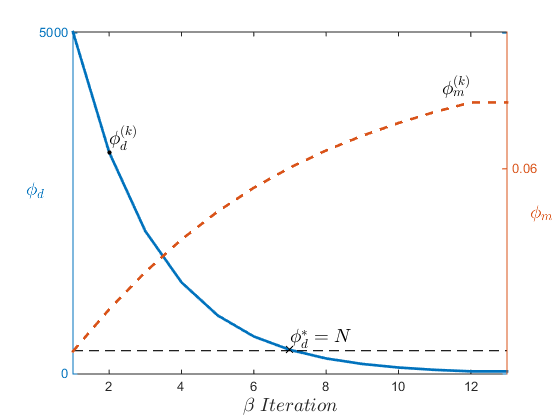
\includegraphics[scale=0.6]{Convergence_curve.png}
\caption{Convergence curve showing the data misfit $\phi_d^{(k)}$ and model norm $\phi_m^{(k)}$ as a function of $\beta$ iterations. The inversion achieves target misfit after the $7^{th}$ iteration, which in this case also corresponds to the point of maximum curvature on the misfit curve. Attempting to further lower the data residual comes at the risk of fitting some of the Gaussian noise.}
\label{fig:Convergence_curve}
\end{figure}

Sections of the recovered susceptibility model from the $7^{th}$ iteration are shown in Figure~\ref{fig:3D_Inv_l2l2_model_INDUCED}. 
Both anomalies are recovered at roughly the right location and at depth. 
As expected from the $l_2$-norm regularization, the model is smoothly varying spatially. Peak susceptibility values are underestimated by roughly $20\%$ due to the smooth constraint.
The model can predict the data well within one standard deviation on average (Fig.~\ref{fig:3D_Inv_l2l2_pred_INDUCED}).
It is worth nothing that there are correlated residuals directly above the magnetic anomaly.
Even though the global misfit criterion is satisfied, there is clearly information in the data that is not being captured.
One option would be to lower the target misfit, but at the risk of fitting some of the random noise.
I tested that strategy on this example, which returned speckly models with isolated susceptibility anomalies near the surface.
A second option would be to manually reduce the uncertainties only over the correlated residuals.
This kind of processing is time consuming and somewhat arbitrary. 
I will argue that the smooth regularization prevents the inversion from fitting the high frequency content.
In Chapter~\ref{ch:Chap4_Mixed_Lpnorm_Regularization} I introduce a compact norm regularization in order to test this hypothesis.

\newpage
\begin{figure}[h!]
\centering
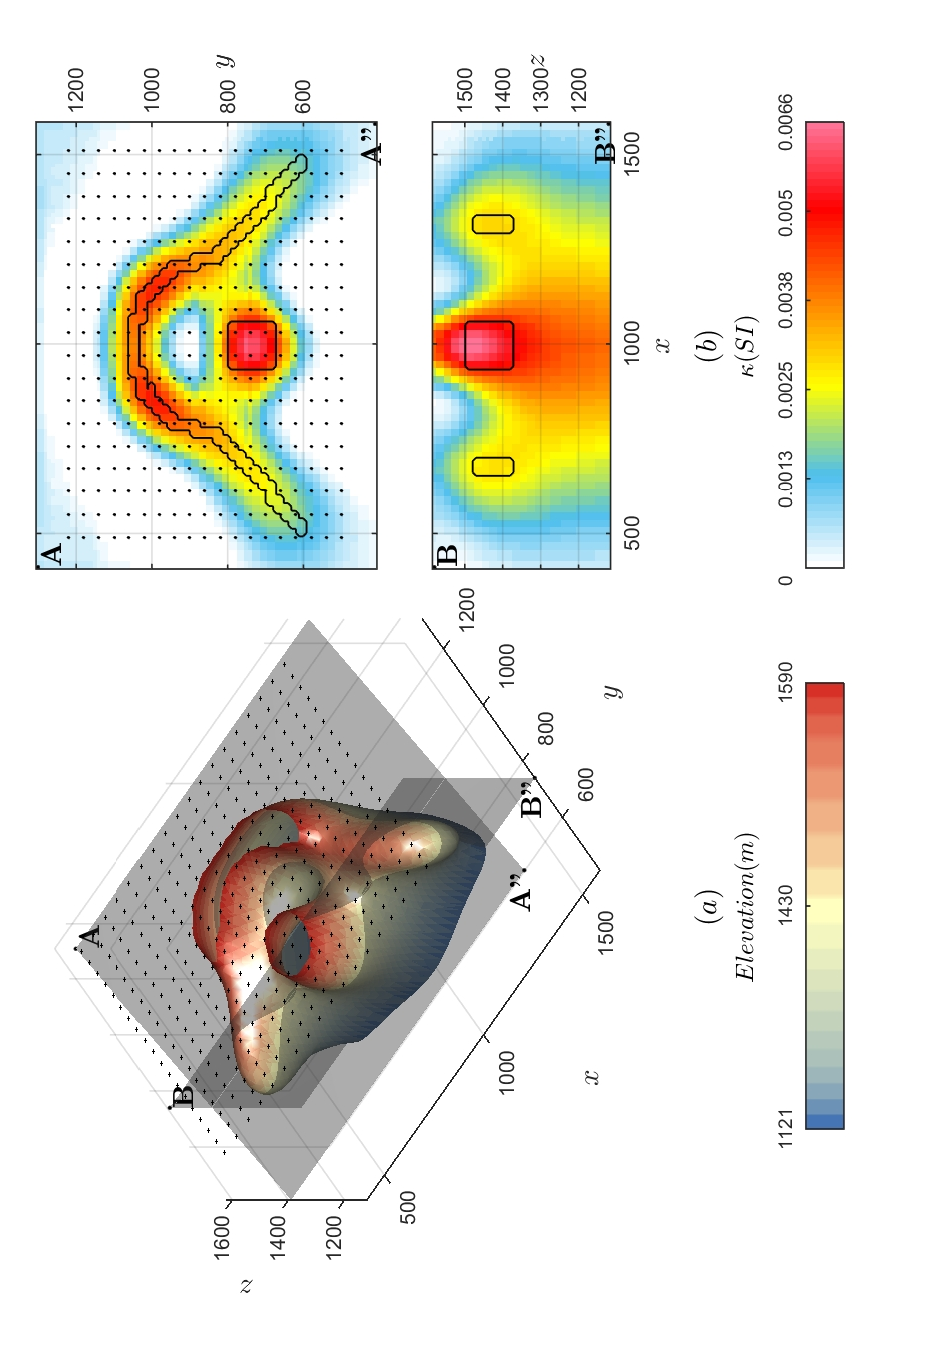
\includegraphics[scale=0.52, angle =270]{3D_Inv_l2l2_model_INDUCED.pdf}
\caption{(a) Iso-surface (0.002 SI) and (b) sections through the recovered susceptibility model for a purely induced response. The model is smooth but recovers the arc and block anomaly at roughly the right depth.}
\label{fig:3D_Inv_l2l2_model_INDUCED}
\end{figure}
\begin{figure}[h!]
\centering
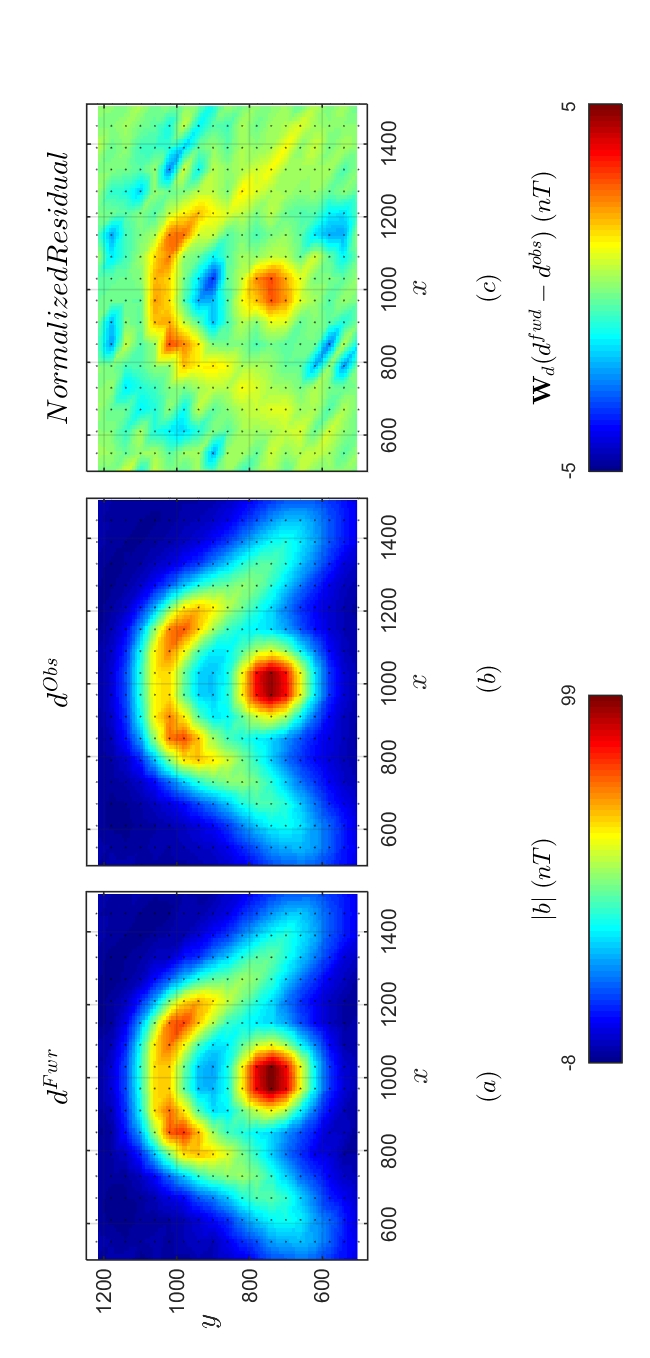
\includegraphics[scale=0.52, angle =270]{3D_Inv_l2l2_pred_INDUCED.pdf}
\caption{ Comparison between (a) observed and (b) predicted data from the recovered susceptibility model. (c) The normalized data residuals appear to be correlated with the location of the magnetic body.}
\label{fig:3D_Inv_l2l2_pred_INDUCED}
\end{figure}

\subsection{Effect of remanent magnetization}
Recent studies have shown that that the assumption of a purely induced response may not be adequate in many geological settings \cite[]{Buchan09, Enkin2014}. 
As presented in \cite{PhDLelievre09}, incorrect assumptions regarding the orientation of magnetization can make the inversion process unreliable.
To simulate this problem, I alter the synthetic model presented in Figure~\ref{fig:3D_Model_INDUCED}. 
I change the orientation of magnetization along the arc-shaped anomaly as shown in Figure~\ref{fig:3D_Model_REMANENT} to simulate a geological folding of a ferromagnetic object.
The magnetization inclination is orientated at $45^{\circ}$ from the horizontal, with variable declinations between $[-45^{\circ}N \;;\;45^{\circ}N]$.
Data are generated from the new magnetization model and corrupted with random Gaussian noise, 1 nT standard deviation ( Fig \ref{fig:3D_Data_REMANENT} ). 
Compared to the purely induced response, the positive anomaly from the arc shifts towards the center while creating a large negative anomaly on the outside boundary of the arc.

Following the same procedure, I invert this new data set while still assuming a purely vertical magnetization direction. 
As presented in Figure \ref{fig:3D_Inv_l2l2_model_REMANENT}, the inversion poorly recovers the location of the arc-shaped body. 
A broad susceptibility anomaly is created on the periphery of the data set, pushing susceptibilities outward in order to account for the large negative data..
The signal from the arc also affects the center block anomaly, that is now recovered deeper than the true location. 
As seen in Figure~\ref{fig:3D_Inv_l2l2_pred_REMANENT}, the inversion algorithm has difficulty fitting the strong negative data. 
In a mineral exploration context, the model presented in \ref{fig:3D_Inv_l2l2_model_REMANENT} could result in false drilling targets \textemdash costly both in time, resources and confidence in geophysical methods.
This is a well known problem in mineral exploration, thus a need for inversion methods that can account for remanence.

\begin{figure}[h!]
\centering
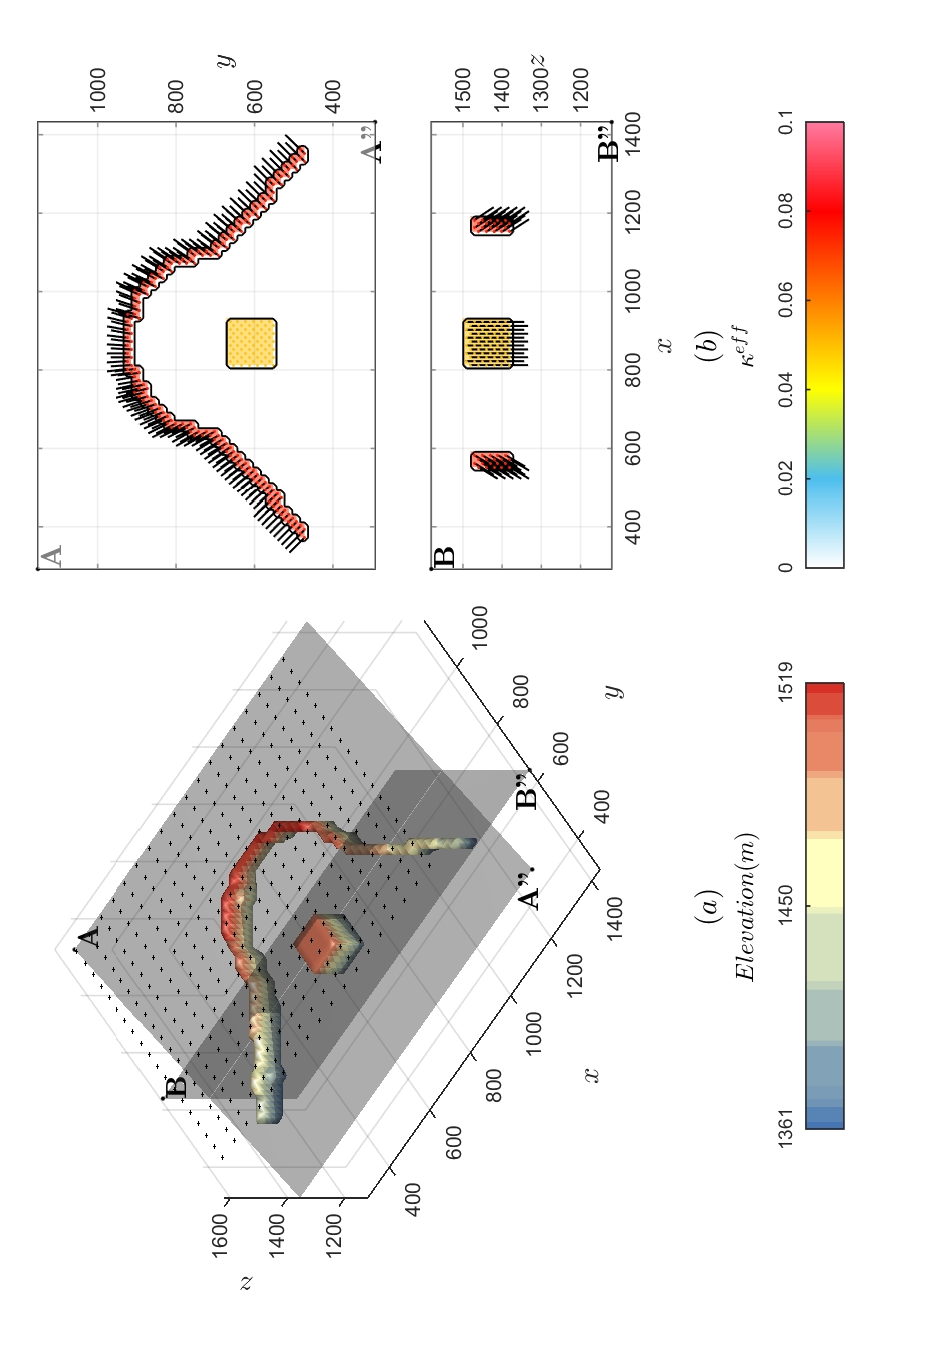
\includegraphics[scale=0.52, angle =270]{3D_Model_REMANENT.pdf}
\caption{ Perspective view and sections through the synthetic magnetization model. The arc-shaped anomaly is magnetized at  $45^{\circ}$ from horizontal and with variable declinations directions between $[-45^{\circ}N \;;\;45^{\circ}N]$. }
%The center block anomaly is still magnetized vertically, parallel to the inducing field.}
\label{fig:3D_Model_REMANENT}
\end{figure}
\begin{figure}[h!]
\centering
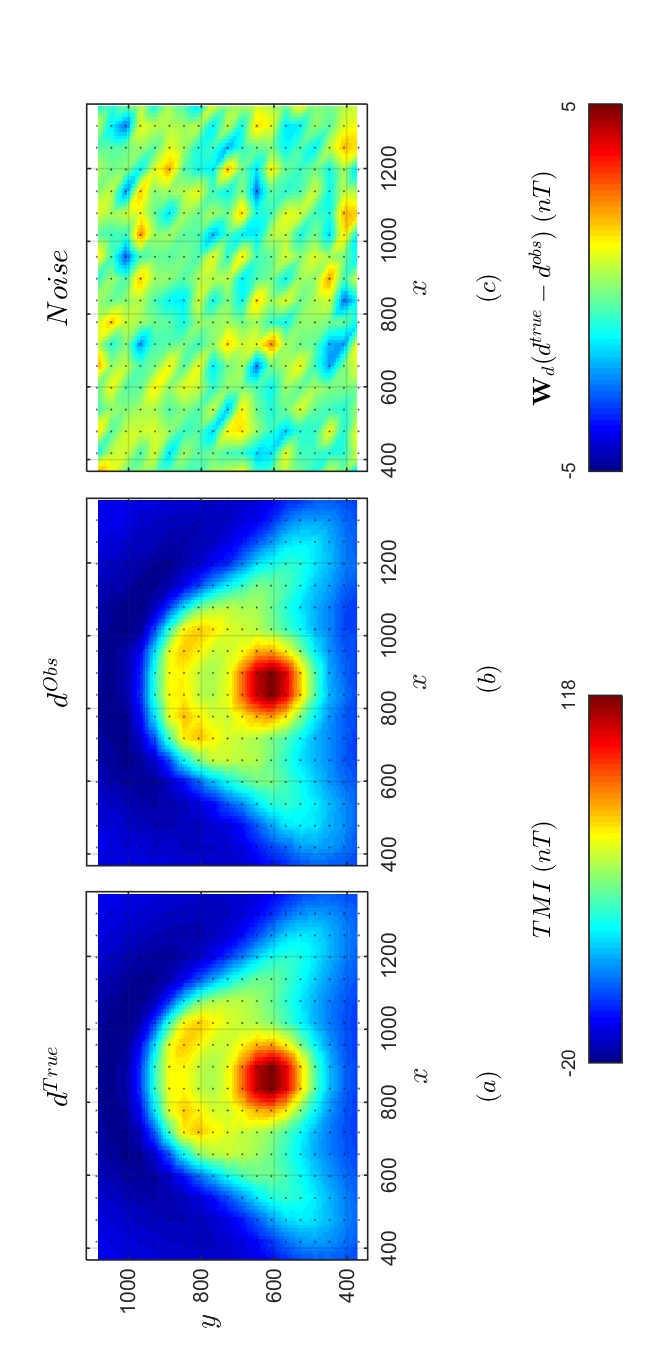
\includegraphics[scale=0.52, angle =270]{3D_Data_REMANENT.pdf}
\caption{ $\bf{(a)}$ Data generated from the synthetic magnetization model. (b) Observed data are corrupted with (c) random Gaussian noise, 1 nT standard deviation.}
\label{fig:3D_Data_REMANENT}
\end{figure}
\begin{figure}[h!]
\centering
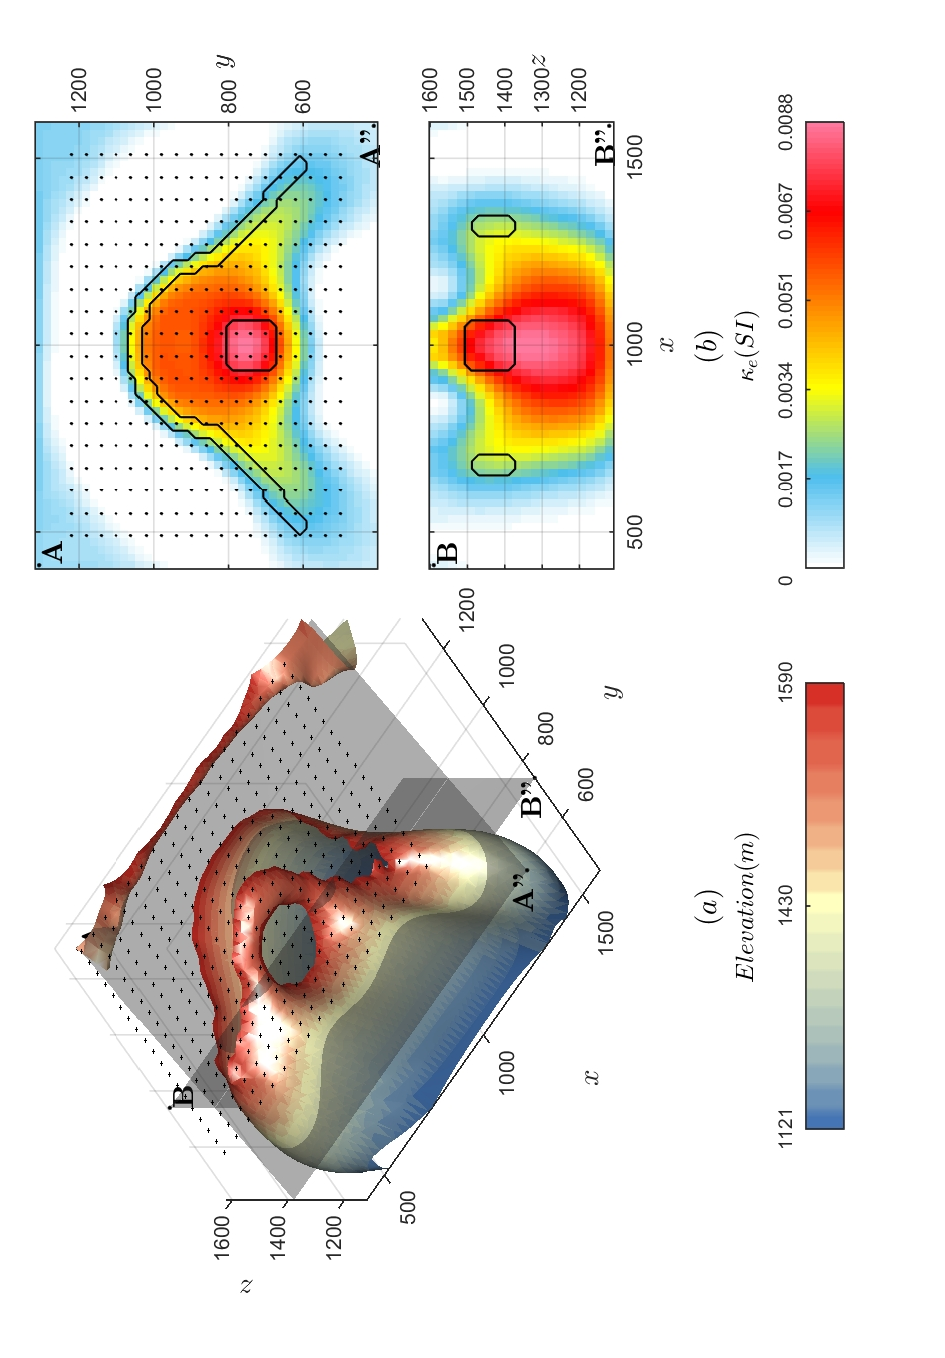
\includegraphics[scale=0.52, angle =270]{3D_Inv_l2l2_model_REMANENT.pdf}
\caption{ (a) Iso-surface (0.002 SI) and (b) sections through the recovered susceptibility model assuming no remanence. The arc-shaped anomaly is poorly recovered and magnetic susceptibilities are pushed at depth and outwards.}
\label{fig:3D_Inv_l2l2_model_REMANENT}
\end{figure}
\begin{figure}[h!]
\centering
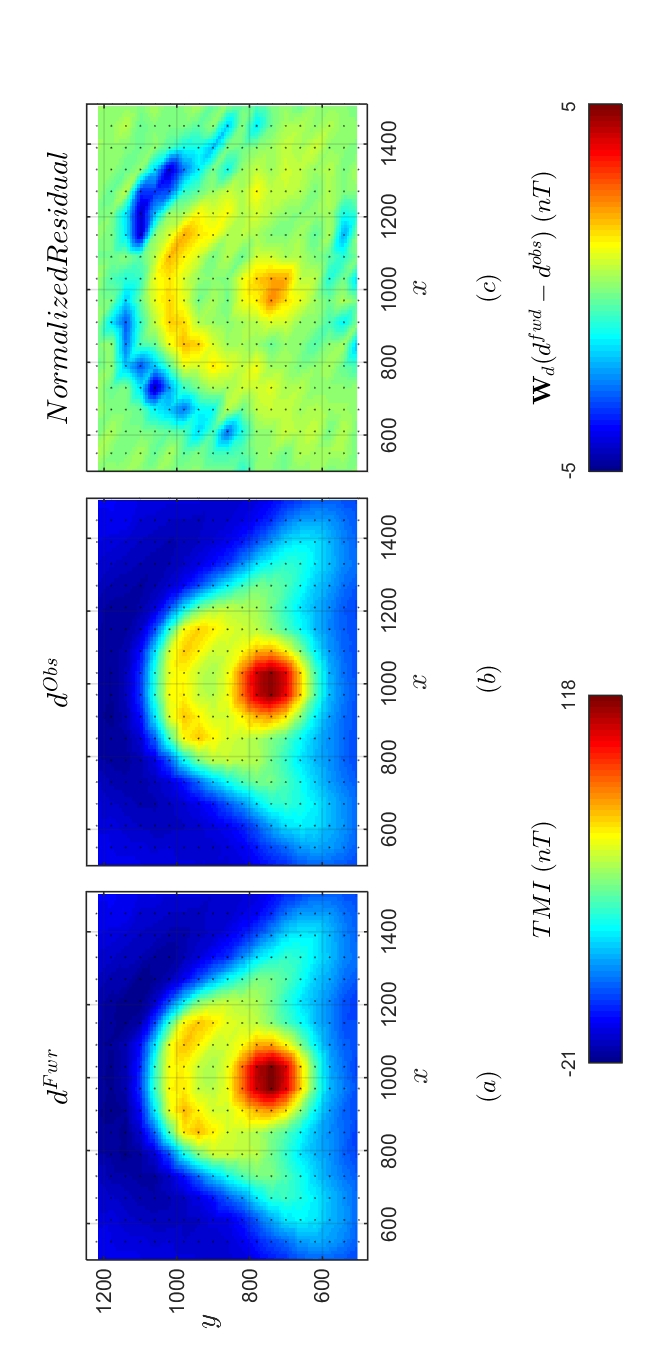
\includegraphics[scale=0.52, angle =270]{3D_Inv_l2l2_pred_REMANENT.pdf}
\caption{Comparison between (a) observed and (b) predicted data from the recovered susceptibility model assuming a purely induced response. (c) The inversion has a harder time fitting the large negative fields along the arc.}
\label{fig:3D_Inv_l2l2_pred_REMANENT}
\end{figure}

\newpage
\section{Magnetic vector inversion}
As shown in the previous example, the assumption of a purely induced magnetization direction has its limitations. In his PhD thesis, \cite{PhDLelievre09} introduces a Magnetization Vector Inversion (MVI) procedure in order to recover both the location and orientation of magnetization. From the general expression for the magnetic field of a prism in \ref{b_explicit}, the forward problem is formulated as:
\begin{equation}\label{MVI_1d}
	\vec{b} = \mathbf{T}\cdot \vec M_p +  \mathbf{T}\cdot \vec M_s +  \mathbf{T}\cdot \vec M_t\;,
\end{equation}
where I define three orthogonal components of magnetization. The primary $\hat{p}$ component is set to be aligned with the inducing field,  the second $\hat{s}$ component has the same azimuth as the primary but is rotated $90^{\circ}$ in inclination. The third component $\hat{t}$ lies on the $xy$-plane and perpendicular to  $\hat{p}$ and $\hat{s}$.
I define the transformation from Cartesian to \{p,s,t\} coordinate system by a double rotation such that:
\begin{equation} 
	\begin{bmatrix} \hat{{p}} & \hat{{s}} & \hat{{t}} \end{bmatrix} = \mathbf{R}_z ({\theta}) \; \mathbf{R}_x ({\phi}) 
	\begin{bmatrix}
	 0 & 0 & 1\\
	1 & 0 & 0 \\
	0 & 1 & 0
	\end{bmatrix}\;,
\end{equation}
where $\theta$ and $\phi$ are the declination and inclination of the inducing field as defined in a Cartesian coordinate, positive counter-clockwise. 
For an inducing field $\vec H_0$ oriented $0^{\circ} I$, $0^{\circ} D$, the components of magnetization $\hat p, \; \hat s$ and $ \hat t$ would be aligned with the Cartesian components $\hat y, \; \hat z$ and $ \hat x$ respectively. 

For the $b_x$ component of the magnetic field due to a single prism magnetized along the \{p,s,t\} direction can be written as:
\begin{equation}
 b_x = 
\begin{bmatrix}
 Txx  &  Txy & Txz
\end{bmatrix}\;\left(
\begin{bmatrix}
H_{\hat p_x}\\H_{\hat p_y}\\H_{ \hat p_z}
\end{bmatrix} \kappa_p +
\begin{bmatrix}
H_{\hat s_x}\\H_{\hat s_y}\\H_{ \hat s_z}
\end{bmatrix} \kappa_s + 
\begin{bmatrix}
H_{\hat t_x}\\H_{\hat t_y}\\H_{ \hat t_z}
\end{bmatrix} \kappa_t \right) \;,
\end{equation}
and likewise for the $b_y$ and $b_z$ components of the magnetic field.
The magnetic data $\vec {b}$ is now function on three orthogonal components of \emph{effective susceptibility} $\kappa_p, \;\kappa_s$ and $\kappa_t$ and their respective direction of magnetization ${\vec{ H}}_p, \; {\vec{ H}}_s$ and ${\vec{ H}}_t$ defined by the $\{p,s,t\}$ coordinate system such that:
\begin{equation}
\begin{split}
		{\vec{ H}}_p =&  |\vec H_0 |\;  \hat{p}\; \\
		{\vec{ H}}_s =&  |\vec H_0 |\;  \hat{s}\;\\
		{\vec{ H}}_t =&  |\vec H_0 |\; \hat{t}\;\;.
\end{split}
\end{equation}

Just as I did for the magnetic susceptibility problem, I augment the linear system for the magnetic response  of $nc$ magnetized prisms as observed at $N$ data locations.  Equation~\ref{MVI_1d} becomes:
\begin{equation}
\begin{split}
	{b}^{TMA} &= \mathbf{ F} \boldsymbol{\hat \kappa} \\
			&= \mathbf{P\;T}\;\begin{bmatrix} \mathbf{H}_p & \mathbf{H}_s & \mathbf{H}_t \end{bmatrix}
	\begin{bmatrix}
	{\kappa_p} \\
	{\kappa_s} \\
	{\kappa_t} 
	\end{bmatrix} \;.
\end{split}
\end{equation}
where $\mathbf{\hat F} \in \mathbb{R}^{N \times (3nc)}$ has now three times the number of variables as the susceptibility inversion described in \ref{Fwr_susc}. The block diagonal matrices $ \mathbf{H}_p,  \mathbf{H}_s$ and  $\mathbf{H}_t \in \mathbb R^{3nc \times nc}$ relate the three effective susceptibility parameters $\kappa_p, \kappa_s$  and $\kappa_t \in \mathbb{R}^{nc}$ to the system of equation $\mathbf{T}$ in Cartesian coordinates. 

The objective function to be minimized becomes:
 \begin{equation} \label{eq:phi_MVI}
\begin{aligned}
&\phi (\hat\kappa) =  \|\mathbf{W_d (\;F \hat \kappa - d}^{obs}\;)\|_2^2 + \beta \| \mathbf{\hat W}_m\hat \kappa \|^2_2\;.
\end{aligned}
\end{equation}
where the weighting matrices and gradient operators comprised by $\mathbf{\hat W}_m$ are block diagonal matrices such that:
\begin{equation*}
\mathbf{\hat W}_\square = 
		\begin{bmatrix}
			\mathbf{W}_\square 		& \dots  		&  0 \\
			\vdots 		&   	\mathbf{W}_\square	&   \vdots \\
			0 		& 	\dots		& \mathbf{W}_\square
		 \end{bmatrix}
\end{equation*}
\begin{equation*}
\mathbf{\hat G}_\square = 
		\begin{bmatrix}
			\mathbf{G}_\square 		& \dots  		&  0 \\
			\vdots 		&   	\mathbf{G}_\square	&   \vdots \\
			0 		& 	\dots		& \mathbf{G}_\square
		 \end{bmatrix}\;.
\end{equation*}
Each operator is three times the size as those used for the susceptibility inversion.

The inversion process follows the same method as the susceptibility inversion and uses the data presented in Figure \ref{fig:3D_Data_REMANENT}. 
The only difference is that effective susceptibilities are allowed to go negative.
Figure \ref{fig:3D_Inv_l2l2_model_TMVI} presents sections of the recovered magnetization model, with color scale representing the total effective susceptibility $\kappa_e$ where:
\begin{equation}
 \kappa_e = {( \kappa_p^2 + \kappa_s^2 + \kappa_t^2)}^{1/2}\;.
\end{equation}

The inverted model recovers the approximate orientation of magnetization in the block anomaly and part of the arc.
The result is smooth however, making it hard to distinguish the extremities of the arc. 
Effective susceptibilities associated with the center block extend deeper than the true model. 
Large effective susceptibility values are found near the top of the mesh, leaving holes in the iso-surface.

The current inversion strategy may work well in simple cases, or when substantial \emph{a priori} information is provided.
For more general cases, the smooth model presented in Figure \ref{fig:3D_Inv_l2l2_model_TMVI} could lead to false interpretation due to the lack of boundaries.
There is still need to develop a robust algorithm that could reduce the non-uniqueness of the MVI formulation with minimal input required from the user.

\newpage
\begin{figure}[h!]
\centering
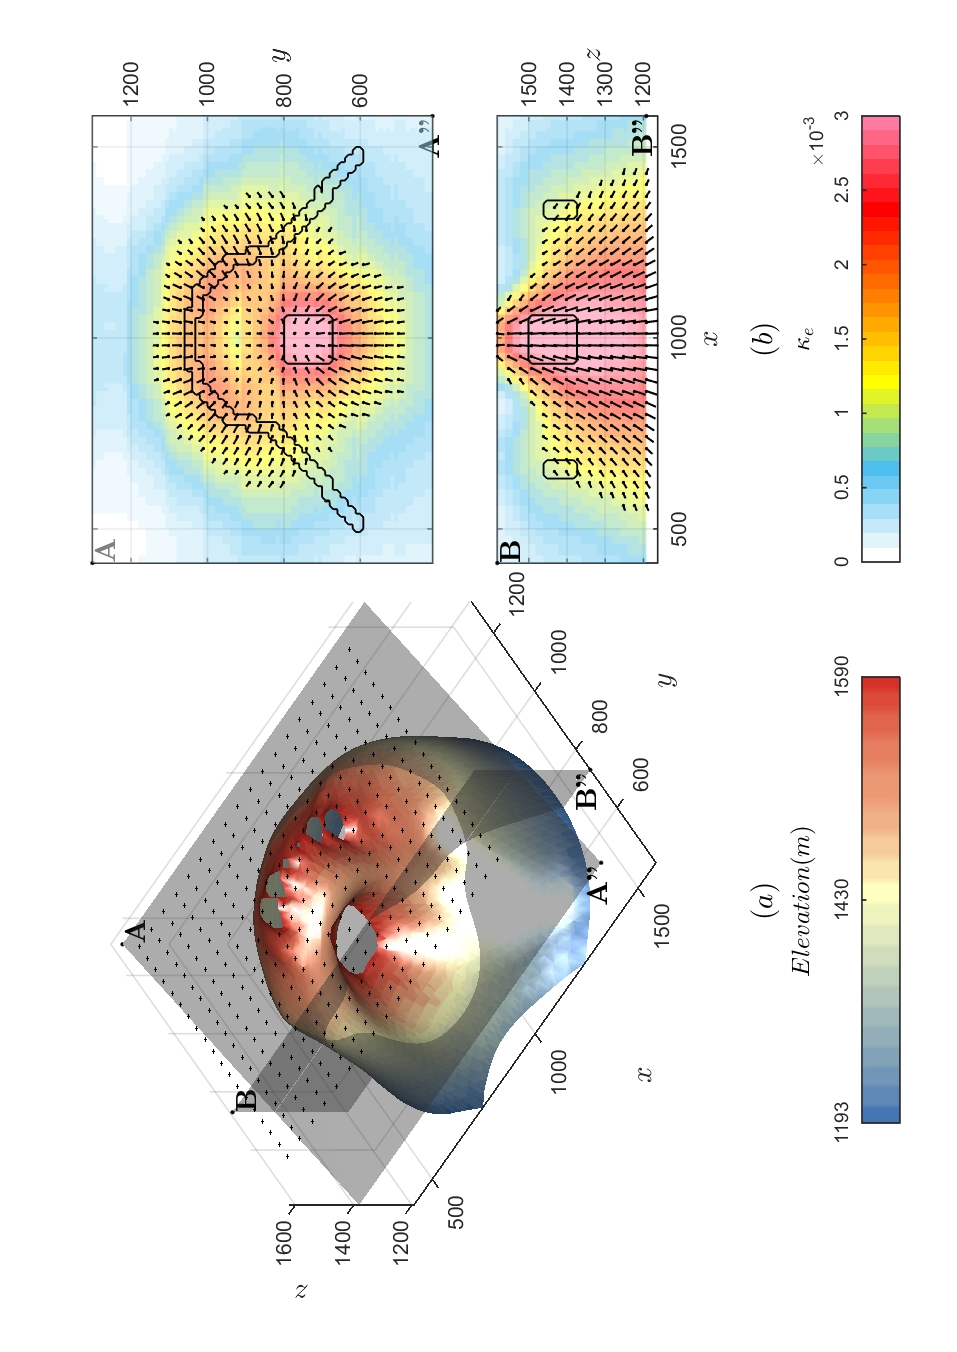
\includegraphics[scale=0.52, angle =270]{3D_Inv_l2l2_model_TMVI.pdf}
\caption{ (a) Iso-surface ($\kappa_e=$0.001) and (b) sections through the recovered magnetization model from the MVI method. The inversion recovers the true orientation of magnetization inside the block, but the thin arc is poorly resolved. }
\label{fig:3D_Inv_l2l2_model_TMVI}
\end{figure}
\begin{figure}[h!]
\centering
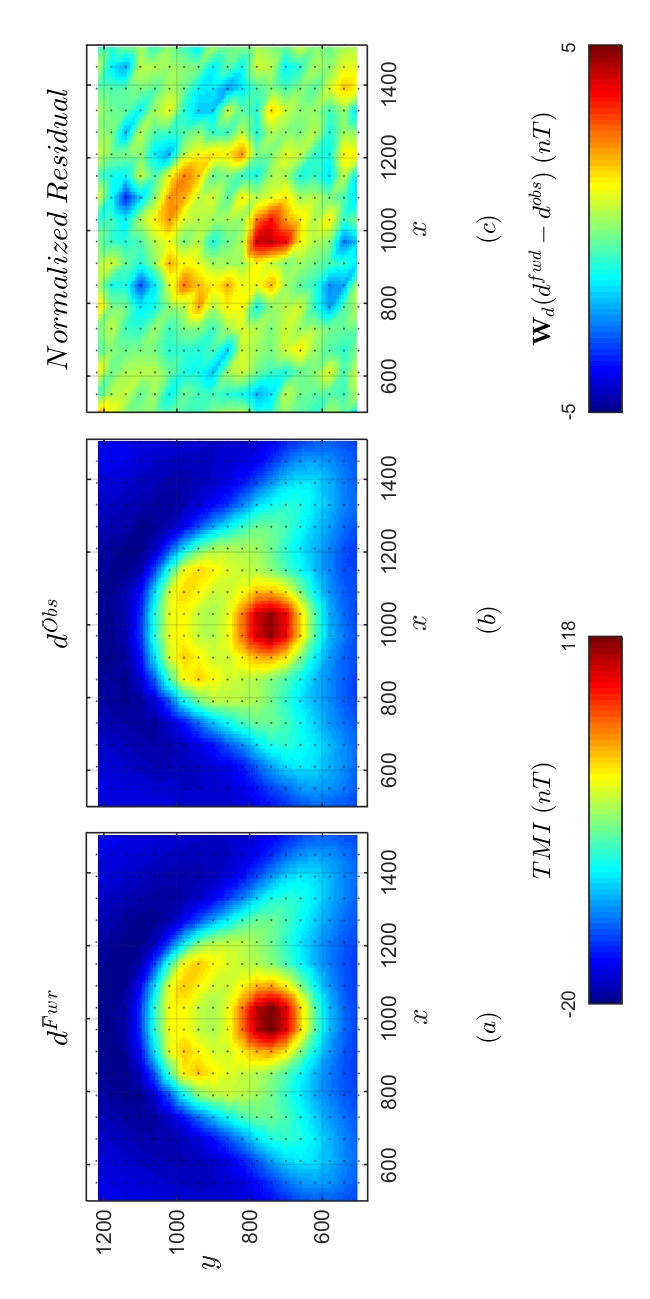
\includegraphics[scale=0.52, angle =270]{3D_Inv_l2l2_pred_TMVI.pdf}
\caption{Comparison between (a) observed and (b) predicted data from the recovered magnetization model from the MVI method. The model can replicate the data at the same level achieved by the purely induced problem.}
\label{fig:3D_Inv_l2l2_pred_TMVI}
\end{figure}

\newpage
\section{Magnetic amplitude inversion}\label{MAI}

The inversion of magnetic quantities, weakly dependent on the magnetization direction, have been proposed as an alternative to the full magnetic vector inversion approach \cite[]{LiShearer10}.
In this section I review the work done by \cite{Shearer05} in inverting magnetic amplitude data.
Amplitude data have the interesting property of being weakly dependent on the orientation of magnetization \cite[]{Nabighian72}, which can be used to get an estimate for the location of magnetized material. I illustrate the idea with a single vertical dipole located at the origin. The magnetic field $\vec {b}$ measured at some distance $\vec r$ can be written as:
 \begin{equation}
\vec {b} = \frac{3\mu_0 m}{{4\pi |r|}^3}\left (\sin{\phi}\cos{\phi}[ \cos{\theta}\:{\hat x} + \sin{\theta}\:{\hat y}] + (\cos^2{\phi} - \frac{1}{3})\:{\hat z} \right) \; ,
\end{equation}
where $\theta$ is the angle on the $xy$-plane, $\phi$ is the angle with respect to the z-axis and $m$ is the dipole moment.
Computing the magnitude of the field yields:
 \begin{equation}
\begin{split}
{|\vec b|} &= \sqrt{ b_x^2 + b_y^2 + bz^2} \\
&= \frac{\mu_0 m}{4\pi|r|^3} \sqrt{3\:\cos^2{(\phi)} + 1} \;.
\end{split}
\end{equation}
The amplitude of the field ${|\vec b|}$ is strongly dependent on the radial distance ${|r|}$, but weakly dependent on $\phi$, the inclination of the dipole. 
If we were to collect magnetic field data at a constant height above the dipole, the location of maximum amplitude would roughly occur above the location of the dipole, and the amplitude of the field would vary by at most a factor two. 
Hence amplitude data may reduce some of the ambiguity related to the horizontal distribution of magnetized material. 

Recall from Chapter~\ref{ch:Chap2_Forward}, I have defined the component of the magnetic field at some location $P$  due to a prism with uniform magnetization $\vec{M}$ as: 
\begin{gather*}
	b_x \: = {[T_{xx} \; T_{xy} \; T_{xz}] }\;  \vec {{M}} \\
	b_y \: ={[T_{yx} \; T_{yy} \; T_{yz}] }\;  \vec {{M}} \\
	b_z \: = {[T_{zx} \; T_{zy} \; T_{zz}]  }\; \vec {{M}} \;,
\end{gather*}
where the forward operator $\mathbf{T}$ maps the components of the magnetic field due to a distribution of magnetized prisms $\vec {{M}}$.
Just as in the MVI method, the magnetization direction is unknown in most cases.
The advantage of working with amplitude data is that the magnetization direction does not have to be known exactly in order to get a good estimate of ${|\vec b|}$. 
Under the assumption that the magnetization vector is in most part parallel to the geomagnetic field direction, equation \ref{Magnetization} can be simplified to:
 \begin{equation*}
\begin{split}
	\vec M &= \kappa(\vec H_0 + \vec H_s) + \vec M_{rem} \\
	&\approx \vec H \; \kappa_{e}\;,
\end{split}
\end{equation*}
where the effective susceptibility $\kappa_{e}$ is a unitless quantity representing the total magnetization of each cell.
Assuming a uniform inducing field $\vec H$, the anomalous magnetic field measurement due to a magnetized cell is approximated by:
 \begin{equation}\label{M_eff}
\begin{split}
%	&M_x = \kappa_e H_{x} \\
%	&M_y = \kappa_e H_{y} \\
%	&M_z = \kappa_e H_{z} \\
\vec b(P) = 
\begin{bmatrix}
b_x\\
b_y\\
b_z\\
\end{bmatrix} &=
 \begin{pmatrix}
       		T_{xx} & T_{xy} & T_{xz}    \\
		T_{yx} & T_{yy} & T_{yz}    \\
		T_{zx} & T_{zy} & T_{zz}           
	\end{pmatrix} 
\begin{bmatrix}
\kappa_e H_{x}\\
\kappa_e H_{y}\\
\kappa_e H_{z}
\end{bmatrix} \\
&=
\begin{bmatrix}
F_x \\
F_y\\
F_z 
\end{bmatrix} \;\kappa_e\;.
\end{split}
\end{equation}
Note the parallel with the $\kappa_{e}$ used in the MVI method to describe the magnetization components $\hat p, \hat s$ and $ \hat t $.
Because the geomagnetic field is generally much larger than any secondary fields, I approximate the magnetization direction to be parallel to the inducing field ($\vec H \simeq \vec H_0$).
%The main difference with the MVI method however is that the amplitude inversion is non-linear with respect to the model parameter $\kappa_{e}$. 
%Assuming a uniform inducing field, equation~\ref{M_eff} can be expanded once again over $N$ magnetic data due to a collection of $nc$ prisms such that:
%\begin{equation}\label{Lin_MAI}
%	\begin{split}
%		\mathbf{b}_x = \left[ H_{0x}\mathbf{T}_{xx} \;+\; H_{0y}\mathbf{T}_{xy}\;+\; H_{0z}\mathbf{T}_{xz} \right] \kappa_e \; \\
%		\mathbf{b}_y = \left[H_{0x}\mathbf{T}_{yx} \;+\; H_{0y}\mathbf{T}_{yy}\;+\; H_{0z}\mathbf{T}_{yz} \right] \kappa_e\; \\
%		\mathbf{b}_z = \left[H_{0x}\mathbf{T}_{zx} \;+\; H_{0y}\mathbf{T}_{zy}\;+\; H_{0z}\mathbf{T}_{zz} \right] \kappa_e\; ,
%	\end{split}
%\end{equation}
%which can also be written in compact form as:
%\begin{equation}\label{Fwr_lBl}
%	\begin{split}
%		\mathbf{b}_x = \mathbf{F}_x \kappa_e \; \\
%		\mathbf{b}_y = \mathbf{F}_y \kappa_e\; \\
%		\mathbf{b}_z = \mathbf{F}_z \kappa_e\; .
%	\end{split}
%\end{equation}
From the linear relation described above, I write the forward calculation of magnetic amplitude data as: 
\begin{equation}\label{MAI_Forward}
	\begin{split}
{|\vec b|} &= 
	\begin{bmatrix}
		{b_x}^2 + {b_y}^2 + {b_z}^2
	\end{bmatrix} ^{1/2} \\
	&= 
	\begin{bmatrix}
		({F_x} \: \boldsymbol{\kappa_e)}^2 \;+
	 ({F_y} \: \boldsymbol{\kappa_e)}^2 \;+
	({F_z} \: \boldsymbol{\kappa_e)}^2
	\end{bmatrix} ^{1/2} \;.
	\end{split}
\end{equation}
Taking the partial derivative in terms of model parameter $\kappa_e$ yields:
\begin{equation}\label{dlBl_dm_derive}
	\begin{split}
\frac{\partial {|\vec b|}}{\partial  \kappa_e} &= 
	\frac{\partial}{\partial \kappa_e} {\left[  {b_x}^2 + {b_y}^2 + {b_z}^2 \right]}^{1/2} \\
	&= \frac{1}{{|\vec b|}} \left[ {{b_x} \frac{\partial{b_x}}{\partial \kappa_e} + {b_y}\frac{\partial{b_y}}{\partial \kappa_e} + {b_z}\frac{\partial{b_z}}{\partial \kappa_e}} \right] \\
&= \frac{1}{{|\vec b|}} \left[ {{b_x} {F}_x + {b_y}{F}_y + {b_z}{F}_z} \right] \;.
	\end{split}
\end{equation}
%Then the sensitivity ${J}_{ij}$ for the $i^{th}$ amplitude data due to the $j^{th}$ prism is given by:
%	\begin{equation}\label{dlBl_dm}
%	{J}_{ij} =\frac{\partial {|\vec b|} }{\partial \kappa_e} = \frac{1}{{|\vec b|}} \left[ {{b_x} {F}_x + {b_y}{F}_y + {b_z}{F}_z} \right] 
%	\end{equation}
The inverse problem is clearly non-linear with respect to the model parameter $\kappa_e$.
A solution is found iteratively as outlined in section \ref{Iterative solver}.
At the $k^{th}$ iteration, the sensitivity relating the $i^{th}$ amplitude data due to the $j^{th}$ prism is given by:
\begin{equation}\label{dlBl_dm_kth}
{J}_{ij} = \frac{\vec b^{(k)}}{{|b^{(k)}|}} \cdot 
\begin{bmatrix}
{F}_x \\
{F}_y \\ 
{F}_z
\end{bmatrix}\;,
\end{equation}
where the magnetic data $\vec b^{(k)}$ is computed from an effective susceptibility found at a previous iteration.
In order to have a Jacobian defined at the first iteration, I choose a small number larger than zero for the starting model ($\kappa^{(0)}=1e-4$).

In mineral exploration, amplitude data must be derived directly from TMA data, which will be covered in Section~\ref{EQS}.
For this synthetic example, amplitude data are generated directly from \ref{MAI_Forward} as I already know the true magnetization model.
Data are corrupted with the same Gaussian noise, 1 nT standard deviation.
Once again, positivity constraints  are enforced on values of effective susceptibility.

Figure \ref{fig:3D_Inv_l2l2_model_kEff} presents the recovered effective susceptibility model after reaching the target misfit.
Compared to the result presented in Figure~\ref{fig:3D_Inv_l2l2_model_REMANENT}, high $\kappa_e$ values are recovered along the arc, and at the right depth inside the center block.
The amplitude model closely resembles the model obtained from the purely induced response obtained in Section~\ref{Induced Mag}.
I note however that the amplitude inversion has the tendency to stretch the model vertically.
This remains an open question.

Comparing the observed and predicted data, the magnetic amplitude inversion fits the data generally well, within one standard deviation as shown in Figure~\ref{fig:3D_Inv_l2l2_pred_kEff}.
Once again, the highest residuals are correlated with the location of the anomaly, which will be tackled in Chapter~\ref{ch:Chap4_Mixed_Lpnorm_Regularization}.

While neither the MVI or amplitude inversion managed to recover the location and orientation of magnetization exactly, both methods brought complementary information. From the MVI method, I am recovering a better estimate of the magnetization direction. With the  amplitude inversion, I get a closer estimate of the true location of magnetic anomalies. 
The next chapter explores different regularization functions in order to further reduce the non-uniqueness of the MVI method.
My goal is to combine those methods into a cooperative inversion work-flow in order to a recover a simpler and more accurate solution.

\newpage
\begin{figure}[h!]
\centering
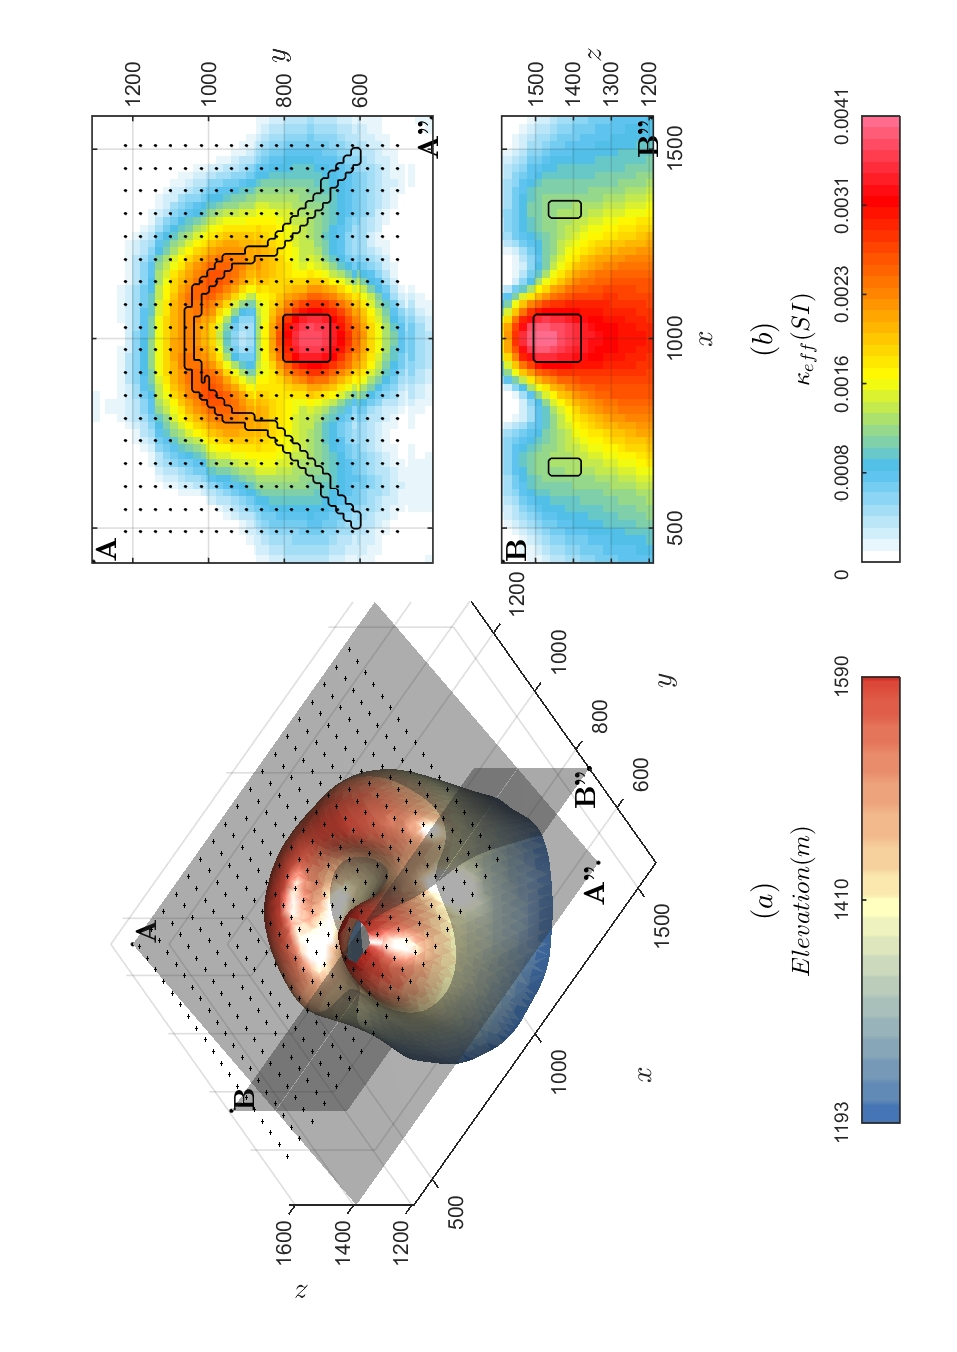
\includegraphics[scale=0.52, angle =270]{3D_Inv_l2l2_model_kEff.pdf}
\caption{ (a) Iso-surface (0.002 SI) and (b) sections through the recovered effective susceptibility model. The arc-shaped and block anomalies are recovered at the right location, but smoothly stretched vertically.}
\label{fig:3D_Inv_l2l2_model_kEff}
\end{figure}
\begin{figure}[h!]
\centering
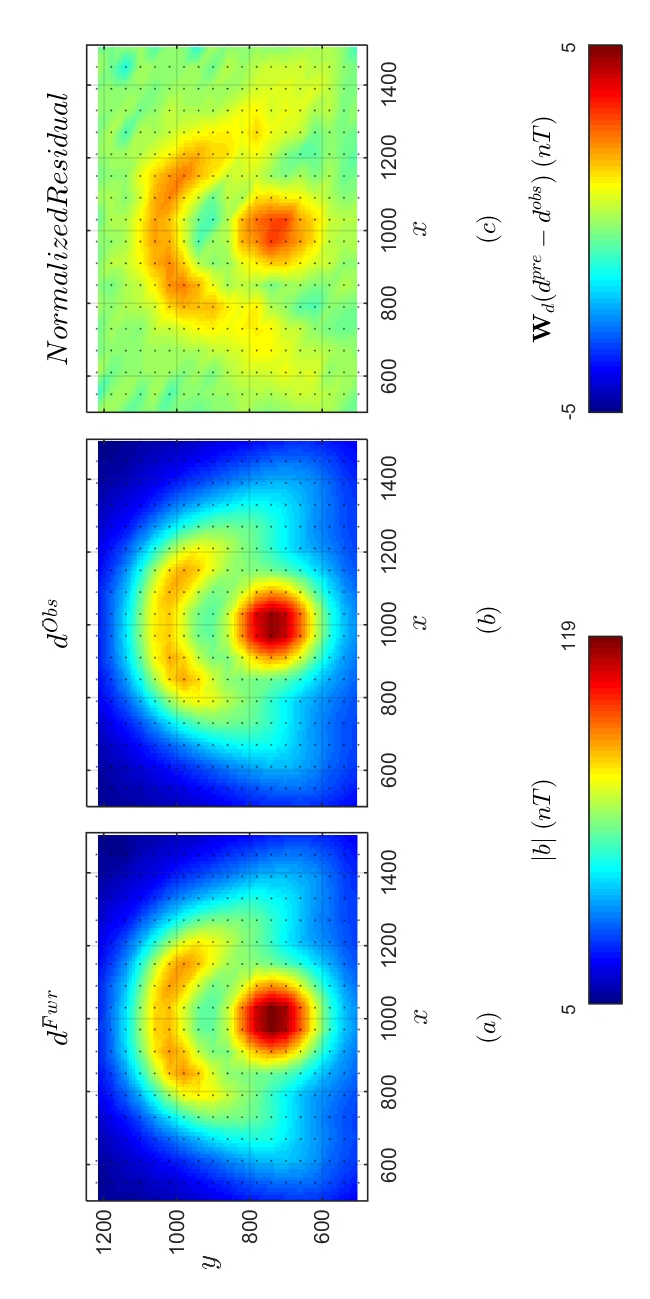
\includegraphics[scale=0.52, angle =270]{3D_Inv_l2l2_pred_kEff.pdf}
\caption{Comparison between (a) observed and (b) predicted data from the recovered effective susceptibility model. The inversion can predict most of the data within one standard deviation.}
\label{fig:3D_Inv_l2l2_pred_kEff}
\end{figure}



\newpage
\section{Equivalent source method}\label{EQS}

The magnetic amplitude inversion method introduced in  \ref{MAI} requires magnetic field components $[b_x,\; b_y,\; b_z]$ in order to calculate amplitude data such that:
\begin{equation}\label{AmpMagData}
\mathbf{|b|} = 
	\begin{bmatrix}
		\mathbf{b_x}^2 + \mathbf{b_y}^2 + \mathbf{b_z}^2
	\end{bmatrix} ^{1/2}  \;.
\end{equation}
While technically possible to measure three-component magnetic data, the vast majority of current and past magnetic surveys consist of TMI measurements.  
This is largely due to the difficulty in determining the location and orientation of three-component receivers. 
Two methods have dominated the literature in order to extract vector components directly from TMI data, either in the frequency domain or by the equivalent source method. 

As demonstrated by \cite{Bhattacharyya64}, TMI data can be expressed as a 2-D Fourier series expansion of the form:
\begin{equation}\label{TMA_Harmonic}
\begin{split}
\mathbf{\vec b}(x,y,z) = \sum_{n=o}^\infty  \sum_{m=o}^\infty \; & e^{{ -2 \pi \; z \; \Big( \frac{m^2}{{L_x}^2} + \frac{n^2}{{L_y}^2} \Big) }^{1/2}} \\
& \Big(A_m \cos{2\pi m \frac{x}{L_x}} + B_m \sin{2\pi m \frac{x}{L_x}}\Big) \\
& \Big(C_m \cos{2\pi n \frac{y}{L_y}} + D_m \sin{2\pi n \frac{y}{L_y}}\Big)\;,
\end{split}
\end{equation}
where $ L_x$ and $L_y$ are the fundamental wavelengths in the $x$ and $y$ directions. The coefficients $A_m$, $B_m$, $C_n$ and $D_n$ are computed from the data for each wavenumber $m$ and $n$. The harmonic representation of the data in \eqref{TMA_Harmonic} can be seen as a product of two functions: an exponential function controlling the amplitude of the signal and an harmonic function for the spatial distribution. 

Converting data from the spatial to the wavenumber domain requires two important assumptions: that the data are located on a plane and distributed over a uniform grid. In most cases however, magnetic surveys are carried along unevenly spaced grids and over rugged topography. Even if acquired on a plane above a  flat topography, the data need to be interpolated and smoothed.
The transformation becomes even more complicated when data are collected at different elevations, as is often the case for airborne surveys with overlapping flight lines.
 
The Equivalent Source method  has been suggested as an alternative to horizontal griding methods \cite[]{Dampney69}. The technique makes use of the inherent ambiguity of potential fields in determining the source location. 
It can be shown that any magnetic response can be explained by an arbitrary distribution of sources. 
In discrete form, an equivalent source model $\mathbf{m_{es}}$ can be calculated from the least-squares problem:
\begin{equation}\label{ES_LeastSquare}
	\underset{m}{\text{min}} \:\| \mathbf{F\;m_{es} - d}\|_2\;.
\end{equation}
As demonstrated by \cite{Dampney69} and later revised by \cite{Li2010}, the distance between the data and the equivalent source is limited by the frequency content of the signal.
Most recent work by \cite{LiNabighian14} addresses striation artifacts when applying a reduction to the pole at low-latitude. They advocate for a positivity constraint formulation and prove the existence of an all-positive equivalent source layer in 2-D.

I replicate the synthetic example presented in \cite{LiNabighian14} as shown in Figure~\ref{fig:ES_Li_True}. 
The model consists of 200 unit cubes with susceptibility of 0.01 SI placed in a non-susceptible background. Data are generated on a plane exactly 1 unit above the anomaly, assuming a purely vertical inducing field of 35,000 nT. Random Gaussian noise with a standard deviation of 1 nT is added to the field components, from which TMI and amplitude data are calculated.
Using the formulation in \cite{LiNabighian14}, I invert for an equivalent source with a positivity constraint. 
The equivalent source layer is placed at a depth that is half the data spacing, in this case at half a unit below the data plane.
Figure \ref{fig:ES_Li_Full_Space} presents the equivalent source layer, as well as the residual between the observed and predicted data. 
All three components of the field, and consequently $\mathbf{|b|}$ data, are well recovered within the noise level. 
Note however that some of the high frequency content related to the edges of the anomaly is lost in the process.

\begin{figure}[h!]
\centering
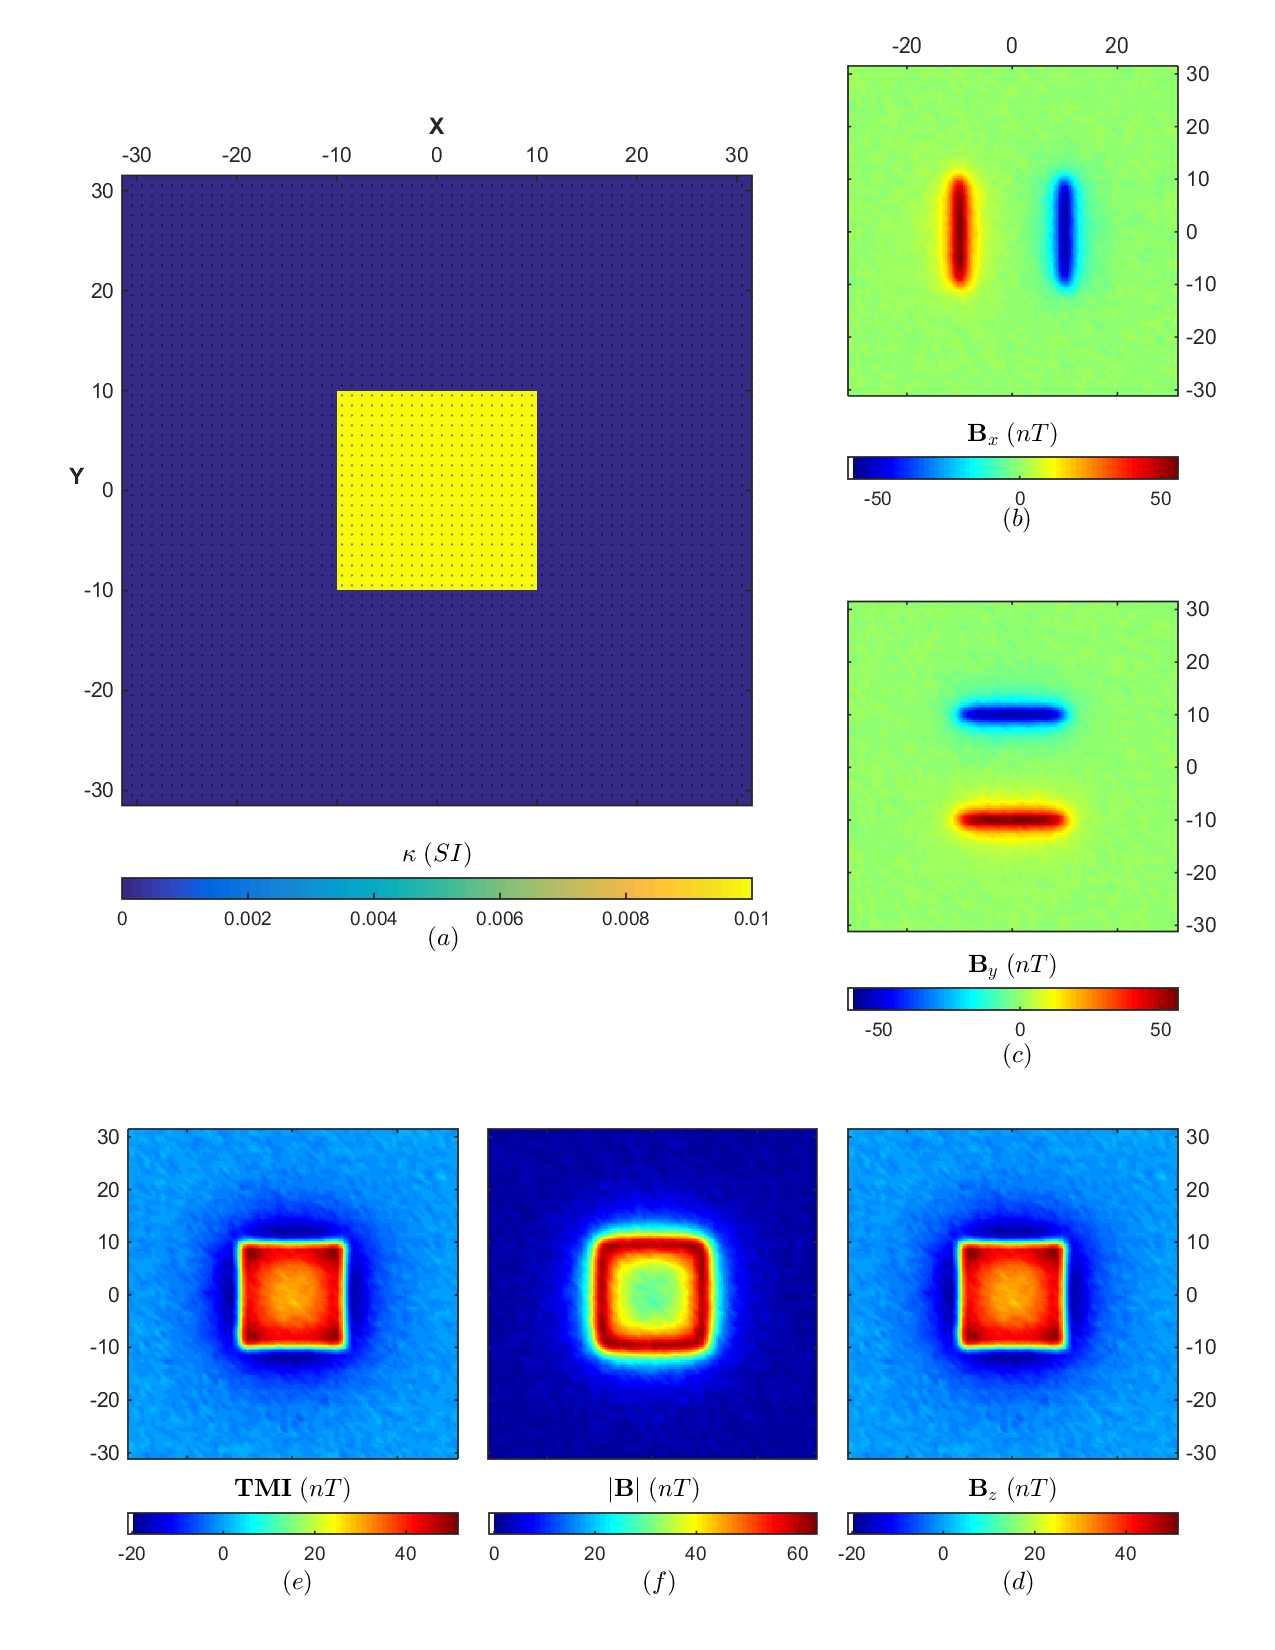
\includegraphics[scale=0.55]{ES_Li_True}
\caption{(a) Synthetic model consisting of $200$ unit cubes of susceptible material in a non-susceptible background. Data are generated on a plane one unit above the source location, assuming a purely vertical inducing field. Various components of the fields are shown in figure (b) to (f). }
\label{fig:ES_Li_True}
\end{figure}

\begin{figure}[h!]
\centering
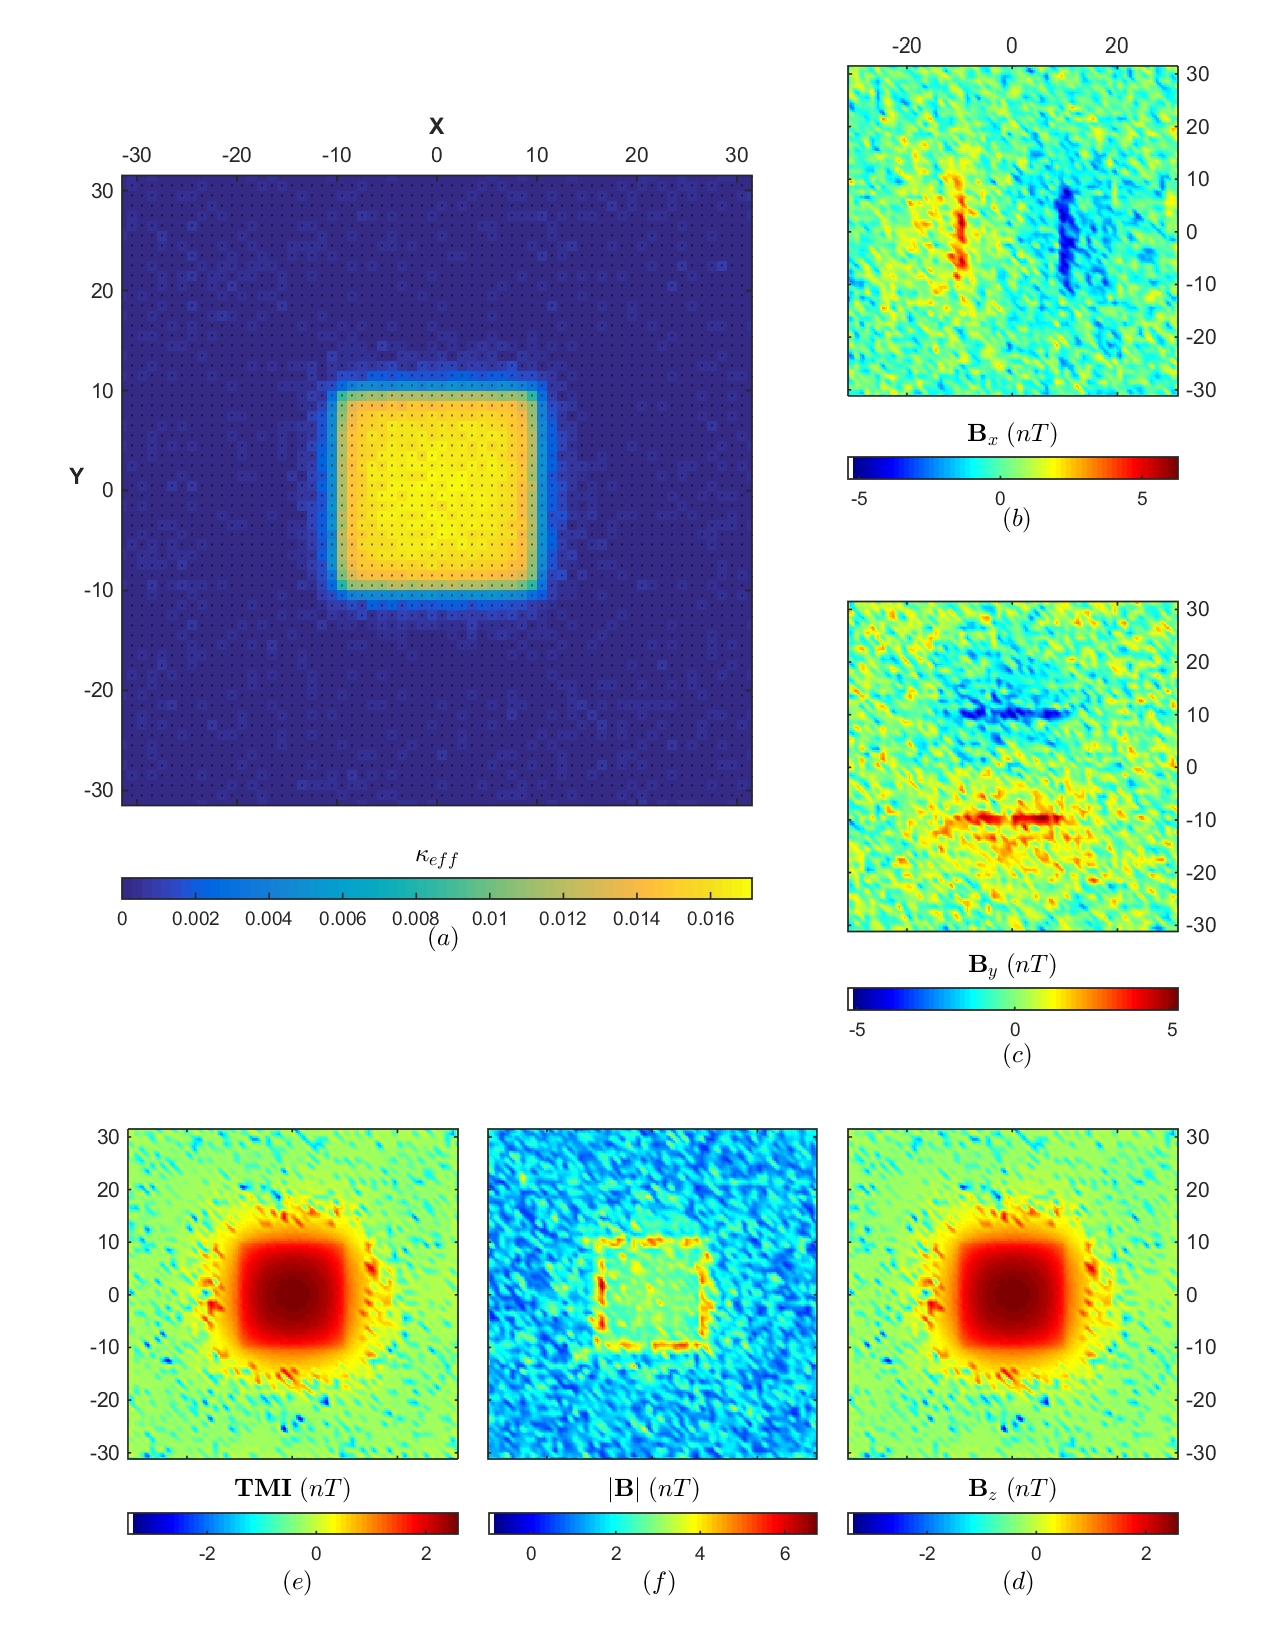
\includegraphics[scale=0.55]{ES_Li_Full_Space}
\caption{(a) Recovered equivalent source layer from TMI data using a positivity constraint. The residuals between observed and predicted data are shown in figure (b) to (f) for various components of the field. Each component is well recovered within the noise level.}
\label{fig:ES_Li_Full_Space}
\end{figure}

\newpage
\subsection{Comment for future research}
While testing the equivalent source method, I experimented on different data distributions to test the stability of the algorithm.
Issues arose in cases where data coverage would partially cover the magnetic anomaly as illustrated in Figure~\ref{fig:ES_Li_CornerOut}.
In this example, a portion of data are removed over one of the corners of the magnetic source.
An equivalent-source layer is then calculated with the same parameters that were previously used for Figure~\ref{fig:ES_Li_Full_Space}.
Large correlated artifacts are created on the $\mathbf{b_x}$ and $\mathbf{b_y}$ component of the field along the missing portion of the data. 
Consequently, a strong narrow anomaly is recovered on $\mathbf{|b|}$ with amplitude in the 40 nT range, well above the noise level.
The same experiment was repeated for various inducing field orientations, transferring the correlated artifacts to other components of the field accordingly.
This suggests some level of ambiguity in the components of the field if the anomalous response is not fully captured by the data.
Such artifacts, if ignored during the inversion process, can have notable consequences on the effective susceptibility model.
It is to my knowledge the first time that this issue is raised, and it will require further research.  
For the remainder of this research project, I continue using the equivalent source method of \cite{LiNabighian14}, but I take special care in removing edge data with large magnetic anomalies.

\begin{figure}[h!]
\centering
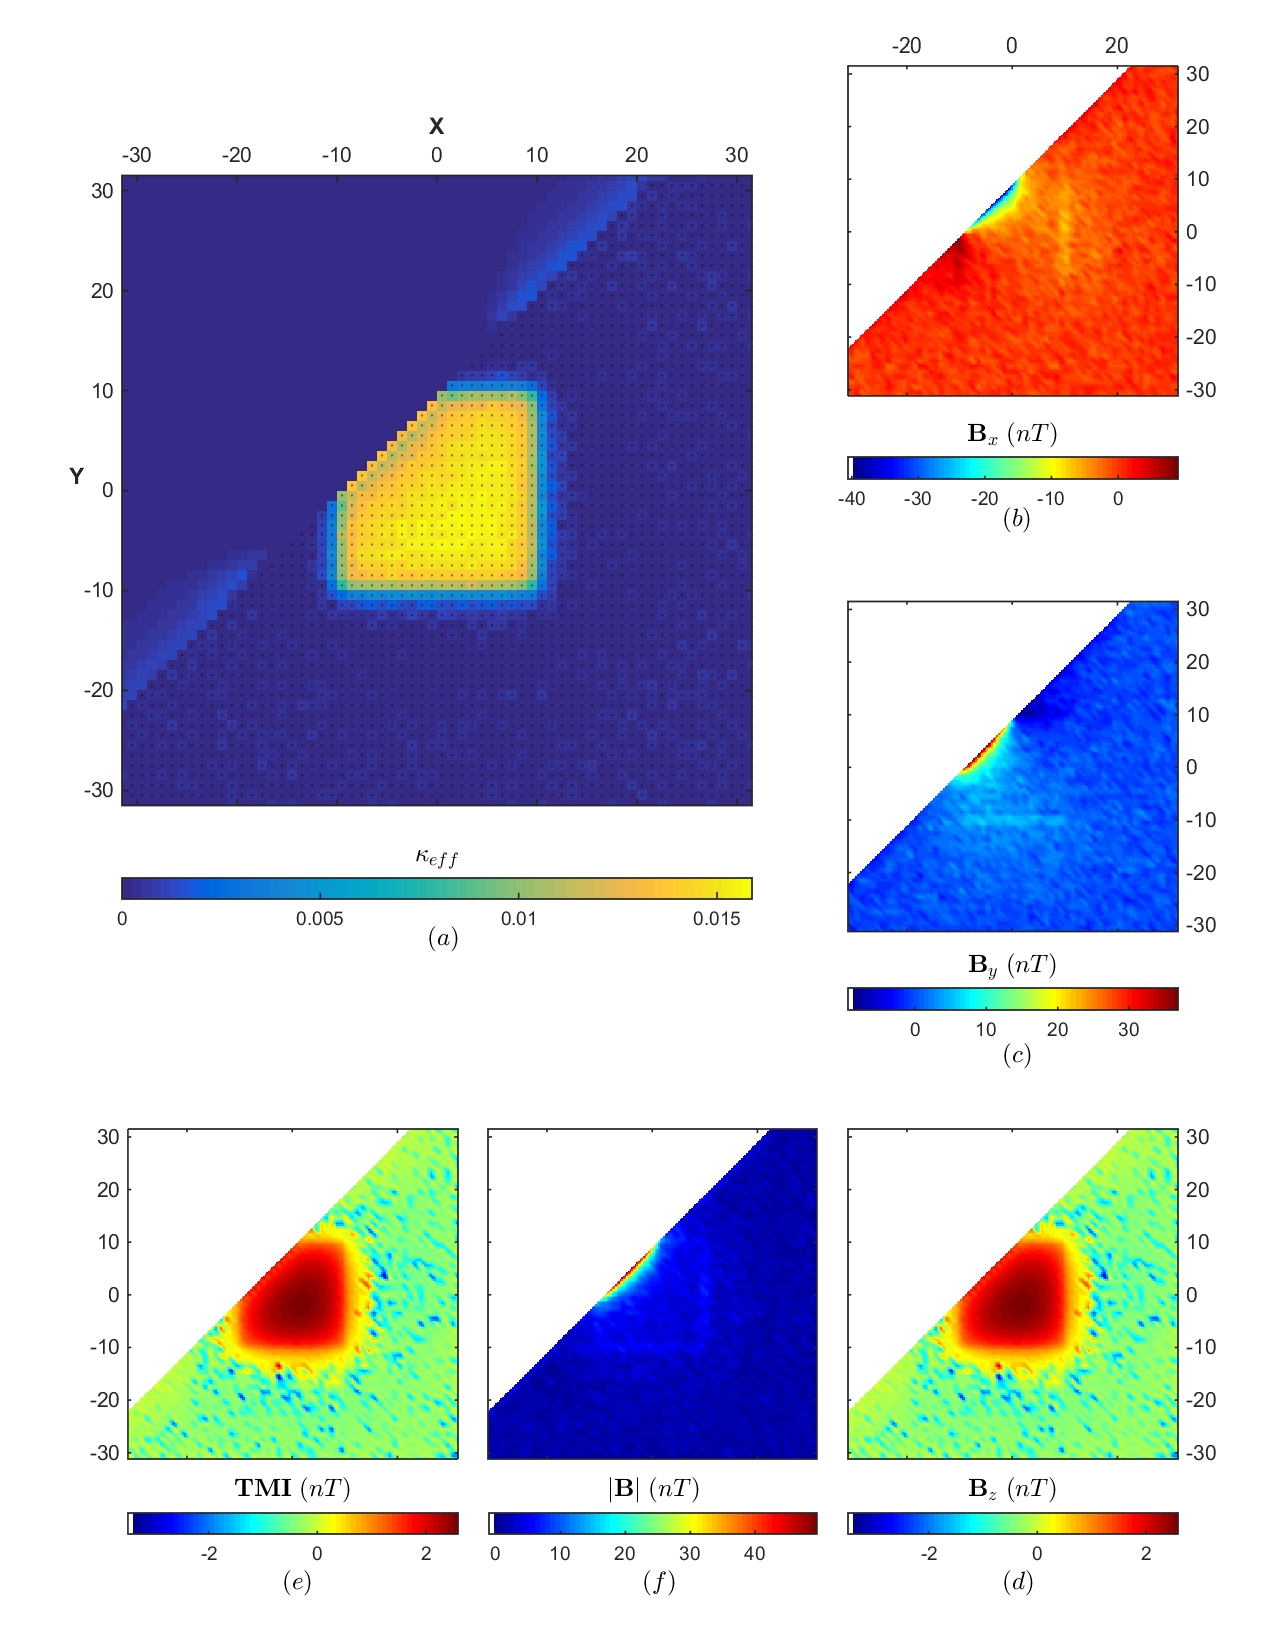
\includegraphics[scale=0.55]{ES_Li_CornerOut}
\caption{(a) Recovered equivalent source layer from TMI data after removing a portion of data over the corner of the magnetic anomaly. The residuals between observed and predicted data are shown in figure (b) to (f) for various components of the field. Note the large correlated artifacts recovered on the $\mathbf{b_x}$, $\mathbf{b_y}$ and $\mathbf{|b|}$ components.}
\label{fig:ES_Li_CornerOut}
\end{figure}


\endinput

